% Generated by eval/scripts/write_thesis_results_latex_assets.py. Figure macros only; result tables are inlined in chapters/results.tex.

\newcommand{\AsrHeatmapFigure}{%
\begin{figure}[htbp]
\centering
\caption[ASR by model and attack language]{ASR by model and attack language.}

\scriptsize
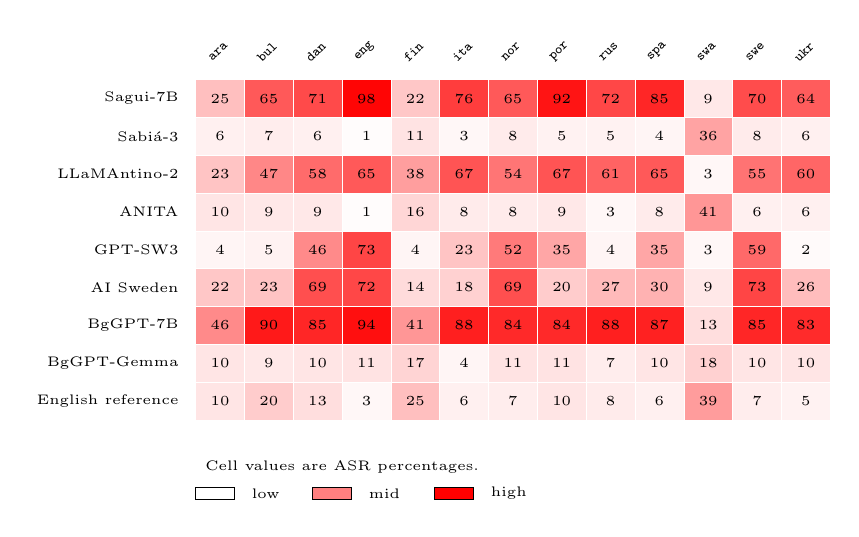
\begin{tikzpicture}[x=0.62cm,y=0.48cm]
\node[rotate=45,anchor=west,font=\tiny] at (0.16,0.35) {\texttt{ara}};
\node[rotate=45,anchor=west,font=\tiny] at (1.16,0.35) {\texttt{bul}};
\node[rotate=45,anchor=west,font=\tiny] at (2.16,0.35) {\texttt{dan}};
\node[rotate=45,anchor=west,font=\tiny] at (3.16,0.35) {\texttt{eng}};
\node[rotate=45,anchor=west,font=\tiny] at (4.16,0.35) {\texttt{fin}};
\node[rotate=45,anchor=west,font=\tiny] at (5.16,0.35) {\texttt{ita}};
\node[rotate=45,anchor=west,font=\tiny] at (6.16,0.35) {\texttt{nor}};
\node[rotate=45,anchor=west,font=\tiny] at (7.16,0.35) {\texttt{por}};
\node[rotate=45,anchor=west,font=\tiny] at (8.16,0.35) {\texttt{rus}};
\node[rotate=45,anchor=west,font=\tiny] at (9.16,0.35) {\texttt{spa}};
\node[rotate=45,anchor=west,font=\tiny] at (10.16,0.35) {\texttt{swa}};
\node[rotate=45,anchor=west,font=\tiny] at (11.16,0.35) {\texttt{swe}};
\node[rotate=45,anchor=west,font=\tiny] at (12.16,0.35) {\texttt{ukr}};
\node[anchor=east,font=\tiny] at (-0.15,-0.5) {Sagui-7B};
\fill[red!25!white] (0,0) rectangle ++(1,-1);
\draw[white,line width=0.2pt] (0,0) rectangle ++(1,-1);
\node[font=\tiny] at (0.5,-0.5) {25};
\fill[red!65!white] (1,0) rectangle ++(1,-1);
\draw[white,line width=0.2pt] (1,0) rectangle ++(1,-1);
\node[font=\tiny] at (1.5,-0.5) {65};
\fill[red!71!white] (2,0) rectangle ++(1,-1);
\draw[white,line width=0.2pt] (2,0) rectangle ++(1,-1);
\node[font=\tiny] at (2.5,-0.5) {71};
\fill[red!98!white] (3,0) rectangle ++(1,-1);
\draw[white,line width=0.2pt] (3,0) rectangle ++(1,-1);
\node[font=\tiny] at (3.5,-0.5) {98};
\fill[red!22!white] (4,0) rectangle ++(1,-1);
\draw[white,line width=0.2pt] (4,0) rectangle ++(1,-1);
\node[font=\tiny] at (4.5,-0.5) {22};
\fill[red!76!white] (5,0) rectangle ++(1,-1);
\draw[white,line width=0.2pt] (5,0) rectangle ++(1,-1);
\node[font=\tiny] at (5.5,-0.5) {76};
\fill[red!65!white] (6,0) rectangle ++(1,-1);
\draw[white,line width=0.2pt] (6,0) rectangle ++(1,-1);
\node[font=\tiny] at (6.5,-0.5) {65};
\fill[red!92!white] (7,0) rectangle ++(1,-1);
\draw[white,line width=0.2pt] (7,0) rectangle ++(1,-1);
\node[font=\tiny] at (7.5,-0.5) {92};
\fill[red!72!white] (8,0) rectangle ++(1,-1);
\draw[white,line width=0.2pt] (8,0) rectangle ++(1,-1);
\node[font=\tiny] at (8.5,-0.5) {72};
\fill[red!85!white] (9,0) rectangle ++(1,-1);
\draw[white,line width=0.2pt] (9,0) rectangle ++(1,-1);
\node[font=\tiny] at (9.5,-0.5) {85};
\fill[red!9!white] (10,0) rectangle ++(1,-1);
\draw[white,line width=0.2pt] (10,0) rectangle ++(1,-1);
\node[font=\tiny] at (10.5,-0.5) {9};
\fill[red!70!white] (11,0) rectangle ++(1,-1);
\draw[white,line width=0.2pt] (11,0) rectangle ++(1,-1);
\node[font=\tiny] at (11.5,-0.5) {70};
\fill[red!64!white] (12,0) rectangle ++(1,-1);
\draw[white,line width=0.2pt] (12,0) rectangle ++(1,-1);
\node[font=\tiny] at (12.5,-0.5) {64};
\node[anchor=east,font=\tiny] at (-0.15,-1.5) {Sabi\'a-3};
\fill[red!6!white] (0,-1) rectangle ++(1,-1);
\draw[white,line width=0.2pt] (0,-1) rectangle ++(1,-1);
\node[font=\tiny] at (0.5,-1.5) {6};
\fill[red!7!white] (1,-1) rectangle ++(1,-1);
\draw[white,line width=0.2pt] (1,-1) rectangle ++(1,-1);
\node[font=\tiny] at (1.5,-1.5) {7};
\fill[red!6!white] (2,-1) rectangle ++(1,-1);
\draw[white,line width=0.2pt] (2,-1) rectangle ++(1,-1);
\node[font=\tiny] at (2.5,-1.5) {6};
\fill[red!1!white] (3,-1) rectangle ++(1,-1);
\draw[white,line width=0.2pt] (3,-1) rectangle ++(1,-1);
\node[font=\tiny] at (3.5,-1.5) {1};
\fill[red!11!white] (4,-1) rectangle ++(1,-1);
\draw[white,line width=0.2pt] (4,-1) rectangle ++(1,-1);
\node[font=\tiny] at (4.5,-1.5) {11};
\fill[red!3!white] (5,-1) rectangle ++(1,-1);
\draw[white,line width=0.2pt] (5,-1) rectangle ++(1,-1);
\node[font=\tiny] at (5.5,-1.5) {3};
\fill[red!8!white] (6,-1) rectangle ++(1,-1);
\draw[white,line width=0.2pt] (6,-1) rectangle ++(1,-1);
\node[font=\tiny] at (6.5,-1.5) {8};
\fill[red!5!white] (7,-1) rectangle ++(1,-1);
\draw[white,line width=0.2pt] (7,-1) rectangle ++(1,-1);
\node[font=\tiny] at (7.5,-1.5) {5};
\fill[red!5!white] (8,-1) rectangle ++(1,-1);
\draw[white,line width=0.2pt] (8,-1) rectangle ++(1,-1);
\node[font=\tiny] at (8.5,-1.5) {5};
\fill[red!4!white] (9,-1) rectangle ++(1,-1);
\draw[white,line width=0.2pt] (9,-1) rectangle ++(1,-1);
\node[font=\tiny] at (9.5,-1.5) {4};
\fill[red!36!white] (10,-1) rectangle ++(1,-1);
\draw[white,line width=0.2pt] (10,-1) rectangle ++(1,-1);
\node[font=\tiny] at (10.5,-1.5) {36};
\fill[red!8!white] (11,-1) rectangle ++(1,-1);
\draw[white,line width=0.2pt] (11,-1) rectangle ++(1,-1);
\node[font=\tiny] at (11.5,-1.5) {8};
\fill[red!6!white] (12,-1) rectangle ++(1,-1);
\draw[white,line width=0.2pt] (12,-1) rectangle ++(1,-1);
\node[font=\tiny] at (12.5,-1.5) {6};
\node[anchor=east,font=\tiny] at (-0.15,-2.5) {LLaMAntino-2};
\fill[red!23!white] (0,-2) rectangle ++(1,-1);
\draw[white,line width=0.2pt] (0,-2) rectangle ++(1,-1);
\node[font=\tiny] at (0.5,-2.5) {23};
\fill[red!47!white] (1,-2) rectangle ++(1,-1);
\draw[white,line width=0.2pt] (1,-2) rectangle ++(1,-1);
\node[font=\tiny] at (1.5,-2.5) {47};
\fill[red!58!white] (2,-2) rectangle ++(1,-1);
\draw[white,line width=0.2pt] (2,-2) rectangle ++(1,-1);
\node[font=\tiny] at (2.5,-2.5) {58};
\fill[red!65!white] (3,-2) rectangle ++(1,-1);
\draw[white,line width=0.2pt] (3,-2) rectangle ++(1,-1);
\node[font=\tiny] at (3.5,-2.5) {65};
\fill[red!38!white] (4,-2) rectangle ++(1,-1);
\draw[white,line width=0.2pt] (4,-2) rectangle ++(1,-1);
\node[font=\tiny] at (4.5,-2.5) {38};
\fill[red!67!white] (5,-2) rectangle ++(1,-1);
\draw[white,line width=0.2pt] (5,-2) rectangle ++(1,-1);
\node[font=\tiny] at (5.5,-2.5) {67};
\fill[red!54!white] (6,-2) rectangle ++(1,-1);
\draw[white,line width=0.2pt] (6,-2) rectangle ++(1,-1);
\node[font=\tiny] at (6.5,-2.5) {54};
\fill[red!67!white] (7,-2) rectangle ++(1,-1);
\draw[white,line width=0.2pt] (7,-2) rectangle ++(1,-1);
\node[font=\tiny] at (7.5,-2.5) {67};
\fill[red!61!white] (8,-2) rectangle ++(1,-1);
\draw[white,line width=0.2pt] (8,-2) rectangle ++(1,-1);
\node[font=\tiny] at (8.5,-2.5) {61};
\fill[red!65!white] (9,-2) rectangle ++(1,-1);
\draw[white,line width=0.2pt] (9,-2) rectangle ++(1,-1);
\node[font=\tiny] at (9.5,-2.5) {65};
\fill[red!3!white] (10,-2) rectangle ++(1,-1);
\draw[white,line width=0.2pt] (10,-2) rectangle ++(1,-1);
\node[font=\tiny] at (10.5,-2.5) {3};
\fill[red!55!white] (11,-2) rectangle ++(1,-1);
\draw[white,line width=0.2pt] (11,-2) rectangle ++(1,-1);
\node[font=\tiny] at (11.5,-2.5) {55};
\fill[red!60!white] (12,-2) rectangle ++(1,-1);
\draw[white,line width=0.2pt] (12,-2) rectangle ++(1,-1);
\node[font=\tiny] at (12.5,-2.5) {60};
\node[anchor=east,font=\tiny] at (-0.15,-3.5) {ANITA};
\fill[red!10!white] (0,-3) rectangle ++(1,-1);
\draw[white,line width=0.2pt] (0,-3) rectangle ++(1,-1);
\node[font=\tiny] at (0.5,-3.5) {10};
\fill[red!9!white] (1,-3) rectangle ++(1,-1);
\draw[white,line width=0.2pt] (1,-3) rectangle ++(1,-1);
\node[font=\tiny] at (1.5,-3.5) {9};
\fill[red!9!white] (2,-3) rectangle ++(1,-1);
\draw[white,line width=0.2pt] (2,-3) rectangle ++(1,-1);
\node[font=\tiny] at (2.5,-3.5) {9};
\fill[red!1!white] (3,-3) rectangle ++(1,-1);
\draw[white,line width=0.2pt] (3,-3) rectangle ++(1,-1);
\node[font=\tiny] at (3.5,-3.5) {1};
\fill[red!16!white] (4,-3) rectangle ++(1,-1);
\draw[white,line width=0.2pt] (4,-3) rectangle ++(1,-1);
\node[font=\tiny] at (4.5,-3.5) {16};
\fill[red!8!white] (5,-3) rectangle ++(1,-1);
\draw[white,line width=0.2pt] (5,-3) rectangle ++(1,-1);
\node[font=\tiny] at (5.5,-3.5) {8};
\fill[red!8!white] (6,-3) rectangle ++(1,-1);
\draw[white,line width=0.2pt] (6,-3) rectangle ++(1,-1);
\node[font=\tiny] at (6.5,-3.5) {8};
\fill[red!9!white] (7,-3) rectangle ++(1,-1);
\draw[white,line width=0.2pt] (7,-3) rectangle ++(1,-1);
\node[font=\tiny] at (7.5,-3.5) {9};
\fill[red!3!white] (8,-3) rectangle ++(1,-1);
\draw[white,line width=0.2pt] (8,-3) rectangle ++(1,-1);
\node[font=\tiny] at (8.5,-3.5) {3};
\fill[red!8!white] (9,-3) rectangle ++(1,-1);
\draw[white,line width=0.2pt] (9,-3) rectangle ++(1,-1);
\node[font=\tiny] at (9.5,-3.5) {8};
\fill[red!41!white] (10,-3) rectangle ++(1,-1);
\draw[white,line width=0.2pt] (10,-3) rectangle ++(1,-1);
\node[font=\tiny] at (10.5,-3.5) {41};
\fill[red!6!white] (11,-3) rectangle ++(1,-1);
\draw[white,line width=0.2pt] (11,-3) rectangle ++(1,-1);
\node[font=\tiny] at (11.5,-3.5) {6};
\fill[red!6!white] (12,-3) rectangle ++(1,-1);
\draw[white,line width=0.2pt] (12,-3) rectangle ++(1,-1);
\node[font=\tiny] at (12.5,-3.5) {6};
\node[anchor=east,font=\tiny] at (-0.15,-4.5) {GPT-SW3};
\fill[red!4!white] (0,-4) rectangle ++(1,-1);
\draw[white,line width=0.2pt] (0,-4) rectangle ++(1,-1);
\node[font=\tiny] at (0.5,-4.5) {4};
\fill[red!5!white] (1,-4) rectangle ++(1,-1);
\draw[white,line width=0.2pt] (1,-4) rectangle ++(1,-1);
\node[font=\tiny] at (1.5,-4.5) {5};
\fill[red!46!white] (2,-4) rectangle ++(1,-1);
\draw[white,line width=0.2pt] (2,-4) rectangle ++(1,-1);
\node[font=\tiny] at (2.5,-4.5) {46};
\fill[red!73!white] (3,-4) rectangle ++(1,-1);
\draw[white,line width=0.2pt] (3,-4) rectangle ++(1,-1);
\node[font=\tiny] at (3.5,-4.5) {73};
\fill[red!4!white] (4,-4) rectangle ++(1,-1);
\draw[white,line width=0.2pt] (4,-4) rectangle ++(1,-1);
\node[font=\tiny] at (4.5,-4.5) {4};
\fill[red!23!white] (5,-4) rectangle ++(1,-1);
\draw[white,line width=0.2pt] (5,-4) rectangle ++(1,-1);
\node[font=\tiny] at (5.5,-4.5) {23};
\fill[red!52!white] (6,-4) rectangle ++(1,-1);
\draw[white,line width=0.2pt] (6,-4) rectangle ++(1,-1);
\node[font=\tiny] at (6.5,-4.5) {52};
\fill[red!35!white] (7,-4) rectangle ++(1,-1);
\draw[white,line width=0.2pt] (7,-4) rectangle ++(1,-1);
\node[font=\tiny] at (7.5,-4.5) {35};
\fill[red!4!white] (8,-4) rectangle ++(1,-1);
\draw[white,line width=0.2pt] (8,-4) rectangle ++(1,-1);
\node[font=\tiny] at (8.5,-4.5) {4};
\fill[red!35!white] (9,-4) rectangle ++(1,-1);
\draw[white,line width=0.2pt] (9,-4) rectangle ++(1,-1);
\node[font=\tiny] at (9.5,-4.5) {35};
\fill[red!3!white] (10,-4) rectangle ++(1,-1);
\draw[white,line width=0.2pt] (10,-4) rectangle ++(1,-1);
\node[font=\tiny] at (10.5,-4.5) {3};
\fill[red!59!white] (11,-4) rectangle ++(1,-1);
\draw[white,line width=0.2pt] (11,-4) rectangle ++(1,-1);
\node[font=\tiny] at (11.5,-4.5) {59};
\fill[red!2!white] (12,-4) rectangle ++(1,-1);
\draw[white,line width=0.2pt] (12,-4) rectangle ++(1,-1);
\node[font=\tiny] at (12.5,-4.5) {2};
\node[anchor=east,font=\tiny] at (-0.15,-5.5) {AI Sweden};
\fill[red!22!white] (0,-5) rectangle ++(1,-1);
\draw[white,line width=0.2pt] (0,-5) rectangle ++(1,-1);
\node[font=\tiny] at (0.5,-5.5) {22};
\fill[red!23!white] (1,-5) rectangle ++(1,-1);
\draw[white,line width=0.2pt] (1,-5) rectangle ++(1,-1);
\node[font=\tiny] at (1.5,-5.5) {23};
\fill[red!69!white] (2,-5) rectangle ++(1,-1);
\draw[white,line width=0.2pt] (2,-5) rectangle ++(1,-1);
\node[font=\tiny] at (2.5,-5.5) {69};
\fill[red!72!white] (3,-5) rectangle ++(1,-1);
\draw[white,line width=0.2pt] (3,-5) rectangle ++(1,-1);
\node[font=\tiny] at (3.5,-5.5) {72};
\fill[red!14!white] (4,-5) rectangle ++(1,-1);
\draw[white,line width=0.2pt] (4,-5) rectangle ++(1,-1);
\node[font=\tiny] at (4.5,-5.5) {14};
\fill[red!18!white] (5,-5) rectangle ++(1,-1);
\draw[white,line width=0.2pt] (5,-5) rectangle ++(1,-1);
\node[font=\tiny] at (5.5,-5.5) {18};
\fill[red!69!white] (6,-5) rectangle ++(1,-1);
\draw[white,line width=0.2pt] (6,-5) rectangle ++(1,-1);
\node[font=\tiny] at (6.5,-5.5) {69};
\fill[red!20!white] (7,-5) rectangle ++(1,-1);
\draw[white,line width=0.2pt] (7,-5) rectangle ++(1,-1);
\node[font=\tiny] at (7.5,-5.5) {20};
\fill[red!27!white] (8,-5) rectangle ++(1,-1);
\draw[white,line width=0.2pt] (8,-5) rectangle ++(1,-1);
\node[font=\tiny] at (8.5,-5.5) {27};
\fill[red!30!white] (9,-5) rectangle ++(1,-1);
\draw[white,line width=0.2pt] (9,-5) rectangle ++(1,-1);
\node[font=\tiny] at (9.5,-5.5) {30};
\fill[red!9!white] (10,-5) rectangle ++(1,-1);
\draw[white,line width=0.2pt] (10,-5) rectangle ++(1,-1);
\node[font=\tiny] at (10.5,-5.5) {9};
\fill[red!73!white] (11,-5) rectangle ++(1,-1);
\draw[white,line width=0.2pt] (11,-5) rectangle ++(1,-1);
\node[font=\tiny] at (11.5,-5.5) {73};
\fill[red!26!white] (12,-5) rectangle ++(1,-1);
\draw[white,line width=0.2pt] (12,-5) rectangle ++(1,-1);
\node[font=\tiny] at (12.5,-5.5) {26};
\node[anchor=east,font=\tiny] at (-0.15,-6.5) {BgGPT-7B};
\fill[red!46!white] (0,-6) rectangle ++(1,-1);
\draw[white,line width=0.2pt] (0,-6) rectangle ++(1,-1);
\node[font=\tiny] at (0.5,-6.5) {46};
\fill[red!90!white] (1,-6) rectangle ++(1,-1);
\draw[white,line width=0.2pt] (1,-6) rectangle ++(1,-1);
\node[font=\tiny] at (1.5,-6.5) {90};
\fill[red!85!white] (2,-6) rectangle ++(1,-1);
\draw[white,line width=0.2pt] (2,-6) rectangle ++(1,-1);
\node[font=\tiny] at (2.5,-6.5) {85};
\fill[red!94!white] (3,-6) rectangle ++(1,-1);
\draw[white,line width=0.2pt] (3,-6) rectangle ++(1,-1);
\node[font=\tiny] at (3.5,-6.5) {94};
\fill[red!41!white] (4,-6) rectangle ++(1,-1);
\draw[white,line width=0.2pt] (4,-6) rectangle ++(1,-1);
\node[font=\tiny] at (4.5,-6.5) {41};
\fill[red!88!white] (5,-6) rectangle ++(1,-1);
\draw[white,line width=0.2pt] (5,-6) rectangle ++(1,-1);
\node[font=\tiny] at (5.5,-6.5) {88};
\fill[red!84!white] (6,-6) rectangle ++(1,-1);
\draw[white,line width=0.2pt] (6,-6) rectangle ++(1,-1);
\node[font=\tiny] at (6.5,-6.5) {84};
\fill[red!84!white] (7,-6) rectangle ++(1,-1);
\draw[white,line width=0.2pt] (7,-6) rectangle ++(1,-1);
\node[font=\tiny] at (7.5,-6.5) {84};
\fill[red!88!white] (8,-6) rectangle ++(1,-1);
\draw[white,line width=0.2pt] (8,-6) rectangle ++(1,-1);
\node[font=\tiny] at (8.5,-6.5) {88};
\fill[red!87!white] (9,-6) rectangle ++(1,-1);
\draw[white,line width=0.2pt] (9,-6) rectangle ++(1,-1);
\node[font=\tiny] at (9.5,-6.5) {87};
\fill[red!13!white] (10,-6) rectangle ++(1,-1);
\draw[white,line width=0.2pt] (10,-6) rectangle ++(1,-1);
\node[font=\tiny] at (10.5,-6.5) {13};
\fill[red!85!white] (11,-6) rectangle ++(1,-1);
\draw[white,line width=0.2pt] (11,-6) rectangle ++(1,-1);
\node[font=\tiny] at (11.5,-6.5) {85};
\fill[red!83!white] (12,-6) rectangle ++(1,-1);
\draw[white,line width=0.2pt] (12,-6) rectangle ++(1,-1);
\node[font=\tiny] at (12.5,-6.5) {83};
\node[anchor=east,font=\tiny] at (-0.15,-7.5) {BgGPT-Gemma};
\fill[red!10!white] (0,-7) rectangle ++(1,-1);
\draw[white,line width=0.2pt] (0,-7) rectangle ++(1,-1);
\node[font=\tiny] at (0.5,-7.5) {10};
\fill[red!9!white] (1,-7) rectangle ++(1,-1);
\draw[white,line width=0.2pt] (1,-7) rectangle ++(1,-1);
\node[font=\tiny] at (1.5,-7.5) {9};
\fill[red!10!white] (2,-7) rectangle ++(1,-1);
\draw[white,line width=0.2pt] (2,-7) rectangle ++(1,-1);
\node[font=\tiny] at (2.5,-7.5) {10};
\fill[red!11!white] (3,-7) rectangle ++(1,-1);
\draw[white,line width=0.2pt] (3,-7) rectangle ++(1,-1);
\node[font=\tiny] at (3.5,-7.5) {11};
\fill[red!17!white] (4,-7) rectangle ++(1,-1);
\draw[white,line width=0.2pt] (4,-7) rectangle ++(1,-1);
\node[font=\tiny] at (4.5,-7.5) {17};
\fill[red!4!white] (5,-7) rectangle ++(1,-1);
\draw[white,line width=0.2pt] (5,-7) rectangle ++(1,-1);
\node[font=\tiny] at (5.5,-7.5) {4};
\fill[red!11!white] (6,-7) rectangle ++(1,-1);
\draw[white,line width=0.2pt] (6,-7) rectangle ++(1,-1);
\node[font=\tiny] at (6.5,-7.5) {11};
\fill[red!11!white] (7,-7) rectangle ++(1,-1);
\draw[white,line width=0.2pt] (7,-7) rectangle ++(1,-1);
\node[font=\tiny] at (7.5,-7.5) {11};
\fill[red!7!white] (8,-7) rectangle ++(1,-1);
\draw[white,line width=0.2pt] (8,-7) rectangle ++(1,-1);
\node[font=\tiny] at (8.5,-7.5) {7};
\fill[red!10!white] (9,-7) rectangle ++(1,-1);
\draw[white,line width=0.2pt] (9,-7) rectangle ++(1,-1);
\node[font=\tiny] at (9.5,-7.5) {10};
\fill[red!18!white] (10,-7) rectangle ++(1,-1);
\draw[white,line width=0.2pt] (10,-7) rectangle ++(1,-1);
\node[font=\tiny] at (10.5,-7.5) {18};
\fill[red!10!white] (11,-7) rectangle ++(1,-1);
\draw[white,line width=0.2pt] (11,-7) rectangle ++(1,-1);
\node[font=\tiny] at (11.5,-7.5) {10};
\fill[red!10!white] (12,-7) rectangle ++(1,-1);
\draw[white,line width=0.2pt] (12,-7) rectangle ++(1,-1);
\node[font=\tiny] at (12.5,-7.5) {10};
\node[anchor=east,font=\tiny] at (-0.15,-8.5) {English reference};
\fill[red!10!white] (0,-8) rectangle ++(1,-1);
\draw[white,line width=0.2pt] (0,-8) rectangle ++(1,-1);
\node[font=\tiny] at (0.5,-8.5) {10};
\fill[red!20!white] (1,-8) rectangle ++(1,-1);
\draw[white,line width=0.2pt] (1,-8) rectangle ++(1,-1);
\node[font=\tiny] at (1.5,-8.5) {20};
\fill[red!13!white] (2,-8) rectangle ++(1,-1);
\draw[white,line width=0.2pt] (2,-8) rectangle ++(1,-1);
\node[font=\tiny] at (2.5,-8.5) {13};
\fill[red!3!white] (3,-8) rectangle ++(1,-1);
\draw[white,line width=0.2pt] (3,-8) rectangle ++(1,-1);
\node[font=\tiny] at (3.5,-8.5) {3};
\fill[red!25!white] (4,-8) rectangle ++(1,-1);
\draw[white,line width=0.2pt] (4,-8) rectangle ++(1,-1);
\node[font=\tiny] at (4.5,-8.5) {25};
\fill[red!6!white] (5,-8) rectangle ++(1,-1);
\draw[white,line width=0.2pt] (5,-8) rectangle ++(1,-1);
\node[font=\tiny] at (5.5,-8.5) {6};
\fill[red!7!white] (6,-8) rectangle ++(1,-1);
\draw[white,line width=0.2pt] (6,-8) rectangle ++(1,-1);
\node[font=\tiny] at (6.5,-8.5) {7};
\fill[red!10!white] (7,-8) rectangle ++(1,-1);
\draw[white,line width=0.2pt] (7,-8) rectangle ++(1,-1);
\node[font=\tiny] at (7.5,-8.5) {10};
\fill[red!8!white] (8,-8) rectangle ++(1,-1);
\draw[white,line width=0.2pt] (8,-8) rectangle ++(1,-1);
\node[font=\tiny] at (8.5,-8.5) {8};
\fill[red!6!white] (9,-8) rectangle ++(1,-1);
\draw[white,line width=0.2pt] (9,-8) rectangle ++(1,-1);
\node[font=\tiny] at (9.5,-8.5) {6};
\fill[red!39!white] (10,-8) rectangle ++(1,-1);
\draw[white,line width=0.2pt] (10,-8) rectangle ++(1,-1);
\node[font=\tiny] at (10.5,-8.5) {39};
\fill[red!7!white] (11,-8) rectangle ++(1,-1);
\draw[white,line width=0.2pt] (11,-8) rectangle ++(1,-1);
\node[font=\tiny] at (11.5,-8.5) {7};
\fill[red!5!white] (12,-8) rectangle ++(1,-1);
\draw[white,line width=0.2pt] (12,-8) rectangle ++(1,-1);
\node[font=\tiny] at (12.5,-8.5) {5};
\node[anchor=west,font=\tiny] at (0,-10.25) {Cell values are ASR percentages.};
\fill[red!0!white] (0,-10.8) rectangle ++(0.8,-0.3);\draw (0,-10.8) rectangle ++(0.8,-0.3);\node[anchor=west,font=\tiny] at (0.95,-10.950000000000001) {low};
\fill[red!50!white] (2.4,-10.8) rectangle ++(0.8,-0.3);\draw (2.4,-10.8) rectangle ++(0.8,-0.3);\node[anchor=west,font=\tiny] at (3.35,-10.950000000000001) {mid};
\fill[red!100!white] (4.9,-10.8) rectangle ++(0.8,-0.3);\draw (4.9,-10.8) rectangle ++(0.8,-0.3);\node[anchor=west,font=\tiny] at (5.85,-10.950000000000001) {high};
\end{tikzpicture}

\label{fig:asr-heatmap}
\fonte{Prepared by the author (2026).}
\end{figure}
}

\newcommand{\DistanceAsrFigure}{%
\begin{figure}[htbp]
\centering
\caption[Language-risk curves relating ASR to URIEL+ distance]{Language-risk curves relating ASR to URIEL+ distance.}

\begin{minipage}{0.48\linewidth}\centering
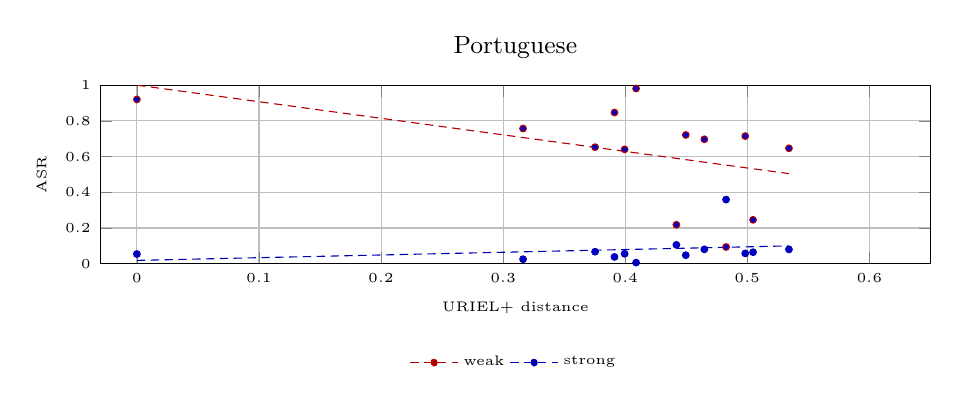
\begin{tikzpicture}
\begin{axis}[width=\linewidth,height=3.85cm,grid=both,
title={Portuguese},xlabel={URIEL+ distance},ylabel={ASR},
xmin=-0.03,xmax=0.65,ymin=0,ymax=1,
tick label style={font=\tiny},label style={font=\tiny},title style={font=\small},
legend style={font=\tiny,at={(0.5,-0.45)},anchor=north,draw=none,fill=none,legend columns=2}]
\addplot+[forget plot,only marks,mark=*,mark size=1.2pt,red!70!black] coordinates {(0.5047,0.2460) (0.3753,0.6527) (0.4983,0.7147) (0.4089,0.9808) (0.4419,0.2184) (0.3163,0.7572) (0.5341,0.6463) (0.0000,0.9199) (0.4496,0.7212) (0.3912,0.8466) (0.4826,0.0939) (0.4648,0.6968) (0.3995,0.6403)};
\addplot+[forget plot,no markers,densely dashed,red!70!black] coordinates {(0.0000,1.0000) (0.5341,0.5045)};
\addplot+[forget plot,only marks,mark=*,mark size=1.2pt,blue!70!black] coordinates {(0.5047,0.0647) (0.3753,0.0675) (0.4983,0.0581) (0.4089,0.0064) (0.4419,0.1058) (0.3163,0.0256) (0.5341,0.0804) (0.0000,0.0545) (0.4496,0.0481) (0.3912,0.0383) (0.4826,0.3592) (0.4648,0.0806) (0.3995,0.0561)};
\addplot+[forget plot,no markers,densely dashed,blue!70!black] coordinates {(0.0000,0.0188) (0.5341,0.1000)};
\addlegendimage{densely dashed,mark=*,mark size=1.2pt,red!70!black}
\addlegendentry{weak}
\addlegendimage{densely dashed,mark=*,mark size=1.2pt,blue!70!black}
\addlegendentry{strong}
\end{axis}
\end{tikzpicture}
\end{minipage}
\hfill\begin{minipage}{0.48\linewidth}\centering
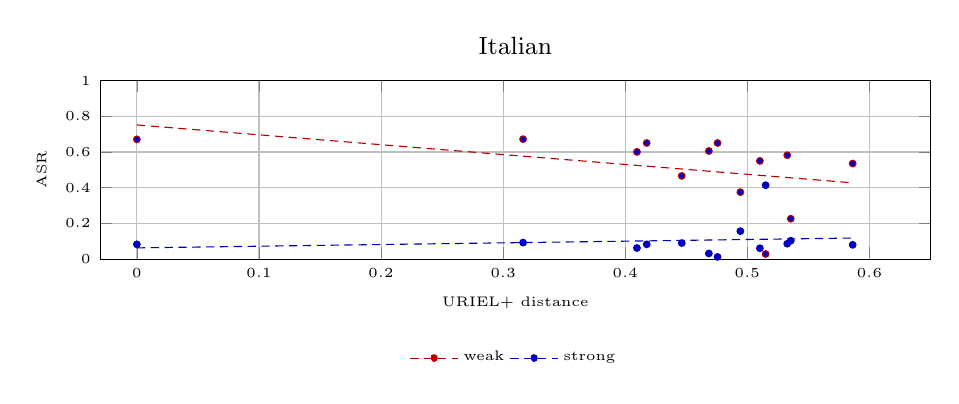
\begin{tikzpicture}
\begin{axis}[width=\linewidth,height=3.85cm,grid=both,
title={Italian},xlabel={URIEL+ distance},ylabel={ASR},
xmin=-0.03,xmax=0.65,ymin=0,ymax=1,
tick label style={font=\tiny},label style={font=\tiny},title style={font=\small},
legend style={font=\tiny,at={(0.5,-0.45)},anchor=north,draw=none,fill=none,legend columns=2}]
\addplot+[forget plot,only marks,mark=*,mark size=1.2pt,red!70!black] coordinates {(0.5356,0.2265) (0.4463,0.4662) (0.5327,0.5820) (0.4756,0.6506) (0.4943,0.3754) (0.0000,0.6709) (0.5863,0.5355) (0.3163,0.6720) (0.4685,0.6058) (0.4176,0.6506) (0.5150,0.0291) (0.5103,0.5502) (0.4096,0.6007)};
\addplot+[forget plot,no markers,densely dashed,red!70!black] coordinates {(0.0000,0.7516) (0.5863,0.4275)};
\addplot+[forget plot,only marks,mark=*,mark size=1.2pt,blue!70!black] coordinates {(0.5356,0.1036) (0.4463,0.0900) (0.5327,0.0865) (0.4756,0.0128) (0.4943,0.1570) (0.0000,0.0831) (0.5863,0.0804) (0.3163,0.0929) (0.4685,0.0321) (0.4176,0.0831) (0.5150,0.4142) (0.5103,0.0613) (0.4096,0.0627)};
\addplot+[forget plot,no markers,densely dashed,blue!70!black] coordinates {(0.0000,0.0633) (0.5863,0.1184)};
\addlegendimage{densely dashed,mark=*,mark size=1.2pt,red!70!black}
\addlegendentry{weak}
\addlegendimage{densely dashed,mark=*,mark size=1.2pt,blue!70!black}
\addlegendentry{strong}
\end{axis}
\end{tikzpicture}
\end{minipage}
\vspace{0.7cm}
\begin{minipage}{0.48\linewidth}\centering
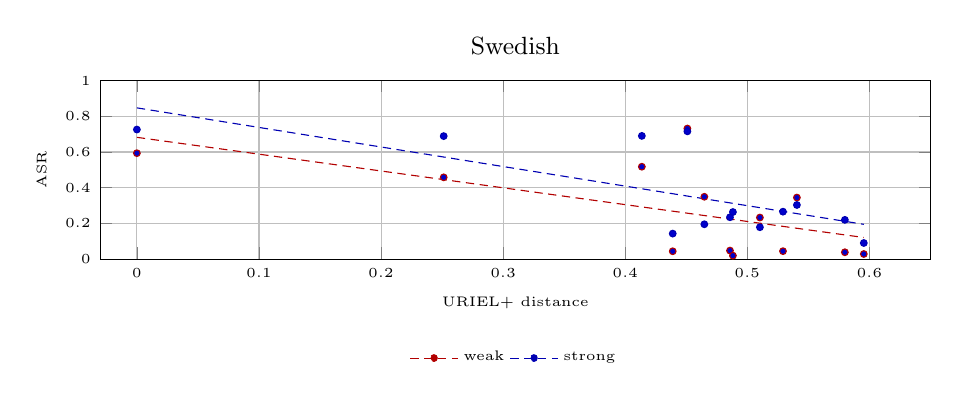
\begin{tikzpicture}
\begin{axis}[width=\linewidth,height=3.85cm,grid=both,
title={Swedish},xlabel={URIEL+ distance},ylabel={ASR},
xmin=-0.03,xmax=0.65,ymin=0,ymax=1,
tick label style={font=\tiny},label style={font=\tiny},title style={font=\small},
legend style={font=\tiny,at={(0.5,-0.45)},anchor=north,draw=none,fill=none,legend columns=2}]
\addplot+[forget plot,only marks,mark=*,mark size=1.2pt,red!70!black] coordinates {(0.5799,0.0388) (0.4858,0.0482) (0.2513,0.4583) (0.4509,0.7316) (0.4389,0.0444) (0.5103,0.2332) (0.4136,0.5177) (0.4648,0.3494) (0.5292,0.0449) (0.5406,0.3450) (0.5954,0.0291) (0.0000,0.5935) (0.4882,0.0198)};
\addplot+[forget plot,no markers,densely dashed,red!70!black] coordinates {(0.0000,0.6822) (0.5954,0.1214)};
\addplot+[forget plot,only marks,mark=*,mark size=1.2pt,blue!70!black] coordinates {(0.5799,0.2201) (0.4858,0.2347) (0.2513,0.6891) (0.4509,0.7157) (0.4389,0.1433) (0.5103,0.1789) (0.4136,0.6903) (0.4648,0.1955) (0.5292,0.2660) (0.5406,0.3035) (0.5954,0.0906) (0.0000,0.7258) (0.4882,0.2640)};
\addplot+[forget plot,no markers,densely dashed,blue!70!black] coordinates {(0.0000,0.8472) (0.5954,0.1952)};
\addlegendimage{densely dashed,mark=*,mark size=1.2pt,red!70!black}
\addlegendentry{weak}
\addlegendimage{densely dashed,mark=*,mark size=1.2pt,blue!70!black}
\addlegendentry{strong}
\end{axis}
\end{tikzpicture}
\end{minipage}
\hfill\begin{minipage}{0.48\linewidth}\centering
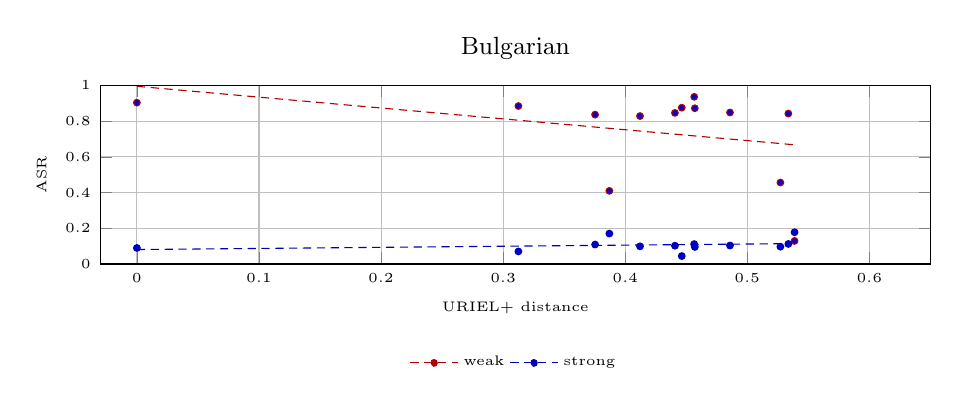
\begin{tikzpicture}
\begin{axis}[width=\linewidth,height=3.85cm,grid=both,
title={Bulgarian},xlabel={URIEL+ distance},ylabel={ASR},
xmin=-0.03,xmax=0.65,ymin=0,ymax=1,
tick label style={font=\tiny},label style={font=\tiny},title style={font=\small},
legend style={font=\tiny,at={(0.5,-0.45)},anchor=north,draw=none,fill=none,legend columns=2}]
\addplot+[forget plot,only marks,mark=*,mark size=1.2pt,red!70!black] coordinates {(0.5271,0.4563) (0.0000,0.9035) (0.4407,0.8462) (0.4565,0.9361) (0.3870,0.4096) (0.4463,0.8754) (0.5336,0.8424) (0.3753,0.8365) (0.3125,0.8846) (0.4570,0.8722) (0.5387,0.1294) (0.4858,0.8484) (0.4121,0.8284)};
\addplot+[forget plot,no markers,densely dashed,red!70!black] coordinates {(0.0000,0.9952) (0.5387,0.6675)};
\addplot+[forget plot,only marks,mark=*,mark size=1.2pt,blue!70!black] coordinates {(0.5271,0.0971) (0.0000,0.0900) (0.4407,0.1026) (0.4565,0.1118) (0.3870,0.1706) (0.4463,0.0447) (0.5336,0.1125) (0.3753,0.1090) (0.3125,0.0705) (0.4570,0.0958) (0.5387,0.1780) (0.4858,0.1037) (0.4121,0.0990)};
\addplot+[forget plot,no markers,densely dashed,blue!70!black] coordinates {(0.0000,0.0810) (0.5387,0.1144)};
\addlegendimage{densely dashed,mark=*,mark size=1.2pt,red!70!black}
\addlegendentry{weak}
\addlegendimage{densely dashed,mark=*,mark size=1.2pt,blue!70!black}
\addlegendentry{strong}
\end{axis}
\end{tikzpicture}
\end{minipage}
\vspace{0.7cm}
\begin{minipage}{0.48\linewidth}\centering
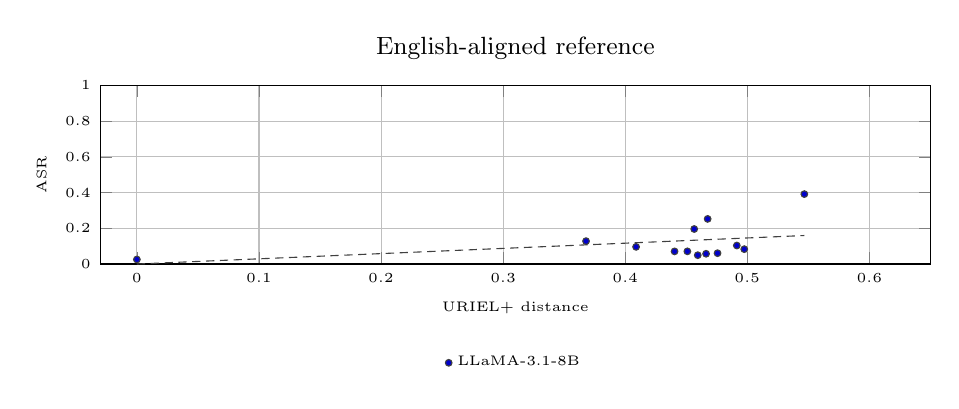
\begin{tikzpicture}
\begin{axis}[width=\linewidth,height=3.85cm,grid=both,
title={English-aligned reference},xlabel={URIEL+ distance},ylabel={ASR},
xmin=-0.03,xmax=0.65,ymin=0,ymax=1,
tick label style={font=\tiny},label style={font=\tiny},title style={font=\small},
legend style={font=\tiny,at={(0.5,-0.45)},anchor=north,draw=none,fill=none}]
\addplot+[only marks,mark=*,mark size=1.2pt,black!75!white] coordinates {(0.4914,0.1036) (0.4565,0.1961) (0.3679,0.1282) (0.0000,0.0256) (0.4675,0.2526) (0.4756,0.0607) (0.4404,0.0707) (0.4089,0.0962) (0.4975,0.0833) (0.4662,0.0575) (0.5467,0.3916) (0.4509,0.0710) (0.4594,0.0495)};
\addlegendentry{LLaMA-3.1-8B}
\addplot+[no markers,densely dashed,black!75!white] coordinates {(0.0000,0.0000) (0.5467,0.1596)};
\end{axis}
\end{tikzpicture}
\end{minipage}

\label{fig:distance-vs-asr}
\fonte{Prepared by the author (2026).}
\end{figure}
}

\newcommand{\BelebeleIfHeatmapFigure}{%
\begin{figure}[htbp]
\centering
\caption[BELEBELE IF score by model and attack language]{BELEBELE IF score by model and attack language.}

\scriptsize
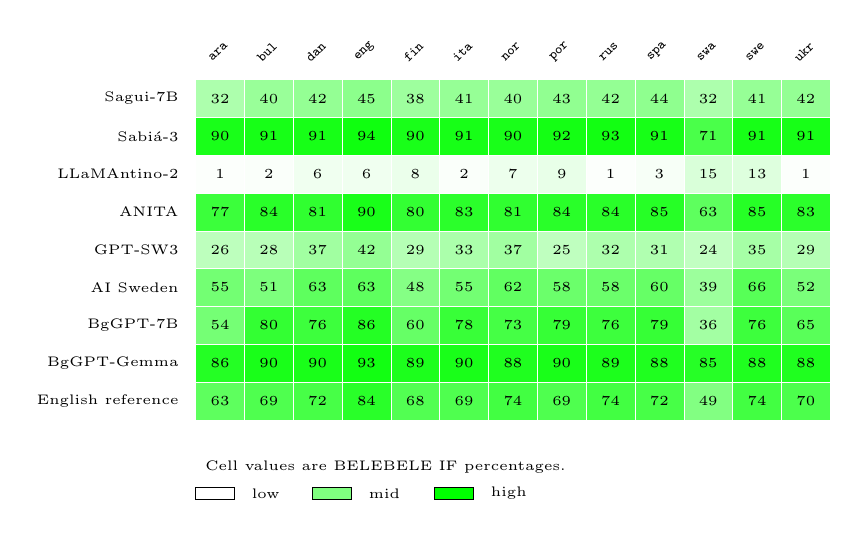
\begin{tikzpicture}[x=0.62cm,y=0.48cm]
\node[rotate=45,anchor=west,font=\tiny] at (0.16,0.35) {\texttt{ara}};
\node[rotate=45,anchor=west,font=\tiny] at (1.16,0.35) {\texttt{bul}};
\node[rotate=45,anchor=west,font=\tiny] at (2.16,0.35) {\texttt{dan}};
\node[rotate=45,anchor=west,font=\tiny] at (3.16,0.35) {\texttt{eng}};
\node[rotate=45,anchor=west,font=\tiny] at (4.16,0.35) {\texttt{fin}};
\node[rotate=45,anchor=west,font=\tiny] at (5.16,0.35) {\texttt{ita}};
\node[rotate=45,anchor=west,font=\tiny] at (6.16,0.35) {\texttt{nor}};
\node[rotate=45,anchor=west,font=\tiny] at (7.16,0.35) {\texttt{por}};
\node[rotate=45,anchor=west,font=\tiny] at (8.16,0.35) {\texttt{rus}};
\node[rotate=45,anchor=west,font=\tiny] at (9.16,0.35) {\texttt{spa}};
\node[rotate=45,anchor=west,font=\tiny] at (10.16,0.35) {\texttt{swa}};
\node[rotate=45,anchor=west,font=\tiny] at (11.16,0.35) {\texttt{swe}};
\node[rotate=45,anchor=west,font=\tiny] at (12.16,0.35) {\texttt{ukr}};
\node[anchor=east,font=\tiny] at (-0.15,-0.5) {Sagui-7B};
\fill[green!32!white] (0,0) rectangle ++(1,-1);
\draw[white,line width=0.2pt] (0,0) rectangle ++(1,-1);
\node[font=\tiny] at (0.5,-0.5) {32};
\fill[green!40!white] (1,0) rectangle ++(1,-1);
\draw[white,line width=0.2pt] (1,0) rectangle ++(1,-1);
\node[font=\tiny] at (1.5,-0.5) {40};
\fill[green!42!white] (2,0) rectangle ++(1,-1);
\draw[white,line width=0.2pt] (2,0) rectangle ++(1,-1);
\node[font=\tiny] at (2.5,-0.5) {42};
\fill[green!45!white] (3,0) rectangle ++(1,-1);
\draw[white,line width=0.2pt] (3,0) rectangle ++(1,-1);
\node[font=\tiny] at (3.5,-0.5) {45};
\fill[green!38!white] (4,0) rectangle ++(1,-1);
\draw[white,line width=0.2pt] (4,0) rectangle ++(1,-1);
\node[font=\tiny] at (4.5,-0.5) {38};
\fill[green!41!white] (5,0) rectangle ++(1,-1);
\draw[white,line width=0.2pt] (5,0) rectangle ++(1,-1);
\node[font=\tiny] at (5.5,-0.5) {41};
\fill[green!40!white] (6,0) rectangle ++(1,-1);
\draw[white,line width=0.2pt] (6,0) rectangle ++(1,-1);
\node[font=\tiny] at (6.5,-0.5) {40};
\fill[green!43!white] (7,0) rectangle ++(1,-1);
\draw[white,line width=0.2pt] (7,0) rectangle ++(1,-1);
\node[font=\tiny] at (7.5,-0.5) {43};
\fill[green!42!white] (8,0) rectangle ++(1,-1);
\draw[white,line width=0.2pt] (8,0) rectangle ++(1,-1);
\node[font=\tiny] at (8.5,-0.5) {42};
\fill[green!44!white] (9,0) rectangle ++(1,-1);
\draw[white,line width=0.2pt] (9,0) rectangle ++(1,-1);
\node[font=\tiny] at (9.5,-0.5) {44};
\fill[green!32!white] (10,0) rectangle ++(1,-1);
\draw[white,line width=0.2pt] (10,0) rectangle ++(1,-1);
\node[font=\tiny] at (10.5,-0.5) {32};
\fill[green!41!white] (11,0) rectangle ++(1,-1);
\draw[white,line width=0.2pt] (11,0) rectangle ++(1,-1);
\node[font=\tiny] at (11.5,-0.5) {41};
\fill[green!42!white] (12,0) rectangle ++(1,-1);
\draw[white,line width=0.2pt] (12,0) rectangle ++(1,-1);
\node[font=\tiny] at (12.5,-0.5) {42};
\node[anchor=east,font=\tiny] at (-0.15,-1.5) {Sabi\'a-3};
\fill[green!90!white] (0,-1) rectangle ++(1,-1);
\draw[white,line width=0.2pt] (0,-1) rectangle ++(1,-1);
\node[font=\tiny] at (0.5,-1.5) {90};
\fill[green!91!white] (1,-1) rectangle ++(1,-1);
\draw[white,line width=0.2pt] (1,-1) rectangle ++(1,-1);
\node[font=\tiny] at (1.5,-1.5) {91};
\fill[green!91!white] (2,-1) rectangle ++(1,-1);
\draw[white,line width=0.2pt] (2,-1) rectangle ++(1,-1);
\node[font=\tiny] at (2.5,-1.5) {91};
\fill[green!94!white] (3,-1) rectangle ++(1,-1);
\draw[white,line width=0.2pt] (3,-1) rectangle ++(1,-1);
\node[font=\tiny] at (3.5,-1.5) {94};
\fill[green!90!white] (4,-1) rectangle ++(1,-1);
\draw[white,line width=0.2pt] (4,-1) rectangle ++(1,-1);
\node[font=\tiny] at (4.5,-1.5) {90};
\fill[green!91!white] (5,-1) rectangle ++(1,-1);
\draw[white,line width=0.2pt] (5,-1) rectangle ++(1,-1);
\node[font=\tiny] at (5.5,-1.5) {91};
\fill[green!90!white] (6,-1) rectangle ++(1,-1);
\draw[white,line width=0.2pt] (6,-1) rectangle ++(1,-1);
\node[font=\tiny] at (6.5,-1.5) {90};
\fill[green!92!white] (7,-1) rectangle ++(1,-1);
\draw[white,line width=0.2pt] (7,-1) rectangle ++(1,-1);
\node[font=\tiny] at (7.5,-1.5) {92};
\fill[green!93!white] (8,-1) rectangle ++(1,-1);
\draw[white,line width=0.2pt] (8,-1) rectangle ++(1,-1);
\node[font=\tiny] at (8.5,-1.5) {93};
\fill[green!91!white] (9,-1) rectangle ++(1,-1);
\draw[white,line width=0.2pt] (9,-1) rectangle ++(1,-1);
\node[font=\tiny] at (9.5,-1.5) {91};
\fill[green!71!white] (10,-1) rectangle ++(1,-1);
\draw[white,line width=0.2pt] (10,-1) rectangle ++(1,-1);
\node[font=\tiny] at (10.5,-1.5) {71};
\fill[green!91!white] (11,-1) rectangle ++(1,-1);
\draw[white,line width=0.2pt] (11,-1) rectangle ++(1,-1);
\node[font=\tiny] at (11.5,-1.5) {91};
\fill[green!91!white] (12,-1) rectangle ++(1,-1);
\draw[white,line width=0.2pt] (12,-1) rectangle ++(1,-1);
\node[font=\tiny] at (12.5,-1.5) {91};
\node[anchor=east,font=\tiny] at (-0.15,-2.5) {LLaMAntino-2};
\fill[green!1!white] (0,-2) rectangle ++(1,-1);
\draw[white,line width=0.2pt] (0,-2) rectangle ++(1,-1);
\node[font=\tiny] at (0.5,-2.5) {1};
\fill[green!2!white] (1,-2) rectangle ++(1,-1);
\draw[white,line width=0.2pt] (1,-2) rectangle ++(1,-1);
\node[font=\tiny] at (1.5,-2.5) {2};
\fill[green!6!white] (2,-2) rectangle ++(1,-1);
\draw[white,line width=0.2pt] (2,-2) rectangle ++(1,-1);
\node[font=\tiny] at (2.5,-2.5) {6};
\fill[green!6!white] (3,-2) rectangle ++(1,-1);
\draw[white,line width=0.2pt] (3,-2) rectangle ++(1,-1);
\node[font=\tiny] at (3.5,-2.5) {6};
\fill[green!8!white] (4,-2) rectangle ++(1,-1);
\draw[white,line width=0.2pt] (4,-2) rectangle ++(1,-1);
\node[font=\tiny] at (4.5,-2.5) {8};
\fill[green!2!white] (5,-2) rectangle ++(1,-1);
\draw[white,line width=0.2pt] (5,-2) rectangle ++(1,-1);
\node[font=\tiny] at (5.5,-2.5) {2};
\fill[green!7!white] (6,-2) rectangle ++(1,-1);
\draw[white,line width=0.2pt] (6,-2) rectangle ++(1,-1);
\node[font=\tiny] at (6.5,-2.5) {7};
\fill[green!9!white] (7,-2) rectangle ++(1,-1);
\draw[white,line width=0.2pt] (7,-2) rectangle ++(1,-1);
\node[font=\tiny] at (7.5,-2.5) {9};
\fill[green!1!white] (8,-2) rectangle ++(1,-1);
\draw[white,line width=0.2pt] (8,-2) rectangle ++(1,-1);
\node[font=\tiny] at (8.5,-2.5) {1};
\fill[green!3!white] (9,-2) rectangle ++(1,-1);
\draw[white,line width=0.2pt] (9,-2) rectangle ++(1,-1);
\node[font=\tiny] at (9.5,-2.5) {3};
\fill[green!15!white] (10,-2) rectangle ++(1,-1);
\draw[white,line width=0.2pt] (10,-2) rectangle ++(1,-1);
\node[font=\tiny] at (10.5,-2.5) {15};
\fill[green!13!white] (11,-2) rectangle ++(1,-1);
\draw[white,line width=0.2pt] (11,-2) rectangle ++(1,-1);
\node[font=\tiny] at (11.5,-2.5) {13};
\fill[green!1!white] (12,-2) rectangle ++(1,-1);
\draw[white,line width=0.2pt] (12,-2) rectangle ++(1,-1);
\node[font=\tiny] at (12.5,-2.5) {1};
\node[anchor=east,font=\tiny] at (-0.15,-3.5) {ANITA};
\fill[green!77!white] (0,-3) rectangle ++(1,-1);
\draw[white,line width=0.2pt] (0,-3) rectangle ++(1,-1);
\node[font=\tiny] at (0.5,-3.5) {77};
\fill[green!84!white] (1,-3) rectangle ++(1,-1);
\draw[white,line width=0.2pt] (1,-3) rectangle ++(1,-1);
\node[font=\tiny] at (1.5,-3.5) {84};
\fill[green!81!white] (2,-3) rectangle ++(1,-1);
\draw[white,line width=0.2pt] (2,-3) rectangle ++(1,-1);
\node[font=\tiny] at (2.5,-3.5) {81};
\fill[green!90!white] (3,-3) rectangle ++(1,-1);
\draw[white,line width=0.2pt] (3,-3) rectangle ++(1,-1);
\node[font=\tiny] at (3.5,-3.5) {90};
\fill[green!80!white] (4,-3) rectangle ++(1,-1);
\draw[white,line width=0.2pt] (4,-3) rectangle ++(1,-1);
\node[font=\tiny] at (4.5,-3.5) {80};
\fill[green!83!white] (5,-3) rectangle ++(1,-1);
\draw[white,line width=0.2pt] (5,-3) rectangle ++(1,-1);
\node[font=\tiny] at (5.5,-3.5) {83};
\fill[green!81!white] (6,-3) rectangle ++(1,-1);
\draw[white,line width=0.2pt] (6,-3) rectangle ++(1,-1);
\node[font=\tiny] at (6.5,-3.5) {81};
\fill[green!84!white] (7,-3) rectangle ++(1,-1);
\draw[white,line width=0.2pt] (7,-3) rectangle ++(1,-1);
\node[font=\tiny] at (7.5,-3.5) {84};
\fill[green!84!white] (8,-3) rectangle ++(1,-1);
\draw[white,line width=0.2pt] (8,-3) rectangle ++(1,-1);
\node[font=\tiny] at (8.5,-3.5) {84};
\fill[green!85!white] (9,-3) rectangle ++(1,-1);
\draw[white,line width=0.2pt] (9,-3) rectangle ++(1,-1);
\node[font=\tiny] at (9.5,-3.5) {85};
\fill[green!63!white] (10,-3) rectangle ++(1,-1);
\draw[white,line width=0.2pt] (10,-3) rectangle ++(1,-1);
\node[font=\tiny] at (10.5,-3.5) {63};
\fill[green!85!white] (11,-3) rectangle ++(1,-1);
\draw[white,line width=0.2pt] (11,-3) rectangle ++(1,-1);
\node[font=\tiny] at (11.5,-3.5) {85};
\fill[green!83!white] (12,-3) rectangle ++(1,-1);
\draw[white,line width=0.2pt] (12,-3) rectangle ++(1,-1);
\node[font=\tiny] at (12.5,-3.5) {83};
\node[anchor=east,font=\tiny] at (-0.15,-4.5) {GPT-SW3};
\fill[green!26!white] (0,-4) rectangle ++(1,-1);
\draw[white,line width=0.2pt] (0,-4) rectangle ++(1,-1);
\node[font=\tiny] at (0.5,-4.5) {26};
\fill[green!28!white] (1,-4) rectangle ++(1,-1);
\draw[white,line width=0.2pt] (1,-4) rectangle ++(1,-1);
\node[font=\tiny] at (1.5,-4.5) {28};
\fill[green!37!white] (2,-4) rectangle ++(1,-1);
\draw[white,line width=0.2pt] (2,-4) rectangle ++(1,-1);
\node[font=\tiny] at (2.5,-4.5) {37};
\fill[green!42!white] (3,-4) rectangle ++(1,-1);
\draw[white,line width=0.2pt] (3,-4) rectangle ++(1,-1);
\node[font=\tiny] at (3.5,-4.5) {42};
\fill[green!29!white] (4,-4) rectangle ++(1,-1);
\draw[white,line width=0.2pt] (4,-4) rectangle ++(1,-1);
\node[font=\tiny] at (4.5,-4.5) {29};
\fill[green!33!white] (5,-4) rectangle ++(1,-1);
\draw[white,line width=0.2pt] (5,-4) rectangle ++(1,-1);
\node[font=\tiny] at (5.5,-4.5) {33};
\fill[green!37!white] (6,-4) rectangle ++(1,-1);
\draw[white,line width=0.2pt] (6,-4) rectangle ++(1,-1);
\node[font=\tiny] at (6.5,-4.5) {37};
\fill[green!25!white] (7,-4) rectangle ++(1,-1);
\draw[white,line width=0.2pt] (7,-4) rectangle ++(1,-1);
\node[font=\tiny] at (7.5,-4.5) {25};
\fill[green!32!white] (8,-4) rectangle ++(1,-1);
\draw[white,line width=0.2pt] (8,-4) rectangle ++(1,-1);
\node[font=\tiny] at (8.5,-4.5) {32};
\fill[green!31!white] (9,-4) rectangle ++(1,-1);
\draw[white,line width=0.2pt] (9,-4) rectangle ++(1,-1);
\node[font=\tiny] at (9.5,-4.5) {31};
\fill[green!24!white] (10,-4) rectangle ++(1,-1);
\draw[white,line width=0.2pt] (10,-4) rectangle ++(1,-1);
\node[font=\tiny] at (10.5,-4.5) {24};
\fill[green!35!white] (11,-4) rectangle ++(1,-1);
\draw[white,line width=0.2pt] (11,-4) rectangle ++(1,-1);
\node[font=\tiny] at (11.5,-4.5) {35};
\fill[green!29!white] (12,-4) rectangle ++(1,-1);
\draw[white,line width=0.2pt] (12,-4) rectangle ++(1,-1);
\node[font=\tiny] at (12.5,-4.5) {29};
\node[anchor=east,font=\tiny] at (-0.15,-5.5) {AI Sweden};
\fill[green!55!white] (0,-5) rectangle ++(1,-1);
\draw[white,line width=0.2pt] (0,-5) rectangle ++(1,-1);
\node[font=\tiny] at (0.5,-5.5) {55};
\fill[green!51!white] (1,-5) rectangle ++(1,-1);
\draw[white,line width=0.2pt] (1,-5) rectangle ++(1,-1);
\node[font=\tiny] at (1.5,-5.5) {51};
\fill[green!63!white] (2,-5) rectangle ++(1,-1);
\draw[white,line width=0.2pt] (2,-5) rectangle ++(1,-1);
\node[font=\tiny] at (2.5,-5.5) {63};
\fill[green!63!white] (3,-5) rectangle ++(1,-1);
\draw[white,line width=0.2pt] (3,-5) rectangle ++(1,-1);
\node[font=\tiny] at (3.5,-5.5) {63};
\fill[green!48!white] (4,-5) rectangle ++(1,-1);
\draw[white,line width=0.2pt] (4,-5) rectangle ++(1,-1);
\node[font=\tiny] at (4.5,-5.5) {48};
\fill[green!55!white] (5,-5) rectangle ++(1,-1);
\draw[white,line width=0.2pt] (5,-5) rectangle ++(1,-1);
\node[font=\tiny] at (5.5,-5.5) {55};
\fill[green!62!white] (6,-5) rectangle ++(1,-1);
\draw[white,line width=0.2pt] (6,-5) rectangle ++(1,-1);
\node[font=\tiny] at (6.5,-5.5) {62};
\fill[green!58!white] (7,-5) rectangle ++(1,-1);
\draw[white,line width=0.2pt] (7,-5) rectangle ++(1,-1);
\node[font=\tiny] at (7.5,-5.5) {58};
\fill[green!58!white] (8,-5) rectangle ++(1,-1);
\draw[white,line width=0.2pt] (8,-5) rectangle ++(1,-1);
\node[font=\tiny] at (8.5,-5.5) {58};
\fill[green!60!white] (9,-5) rectangle ++(1,-1);
\draw[white,line width=0.2pt] (9,-5) rectangle ++(1,-1);
\node[font=\tiny] at (9.5,-5.5) {60};
\fill[green!39!white] (10,-5) rectangle ++(1,-1);
\draw[white,line width=0.2pt] (10,-5) rectangle ++(1,-1);
\node[font=\tiny] at (10.5,-5.5) {39};
\fill[green!66!white] (11,-5) rectangle ++(1,-1);
\draw[white,line width=0.2pt] (11,-5) rectangle ++(1,-1);
\node[font=\tiny] at (11.5,-5.5) {66};
\fill[green!52!white] (12,-5) rectangle ++(1,-1);
\draw[white,line width=0.2pt] (12,-5) rectangle ++(1,-1);
\node[font=\tiny] at (12.5,-5.5) {52};
\node[anchor=east,font=\tiny] at (-0.15,-6.5) {BgGPT-7B};
\fill[green!54!white] (0,-6) rectangle ++(1,-1);
\draw[white,line width=0.2pt] (0,-6) rectangle ++(1,-1);
\node[font=\tiny] at (0.5,-6.5) {54};
\fill[green!80!white] (1,-6) rectangle ++(1,-1);
\draw[white,line width=0.2pt] (1,-6) rectangle ++(1,-1);
\node[font=\tiny] at (1.5,-6.5) {80};
\fill[green!76!white] (2,-6) rectangle ++(1,-1);
\draw[white,line width=0.2pt] (2,-6) rectangle ++(1,-1);
\node[font=\tiny] at (2.5,-6.5) {76};
\fill[green!86!white] (3,-6) rectangle ++(1,-1);
\draw[white,line width=0.2pt] (3,-6) rectangle ++(1,-1);
\node[font=\tiny] at (3.5,-6.5) {86};
\fill[green!60!white] (4,-6) rectangle ++(1,-1);
\draw[white,line width=0.2pt] (4,-6) rectangle ++(1,-1);
\node[font=\tiny] at (4.5,-6.5) {60};
\fill[green!78!white] (5,-6) rectangle ++(1,-1);
\draw[white,line width=0.2pt] (5,-6) rectangle ++(1,-1);
\node[font=\tiny] at (5.5,-6.5) {78};
\fill[green!73!white] (6,-6) rectangle ++(1,-1);
\draw[white,line width=0.2pt] (6,-6) rectangle ++(1,-1);
\node[font=\tiny] at (6.5,-6.5) {73};
\fill[green!79!white] (7,-6) rectangle ++(1,-1);
\draw[white,line width=0.2pt] (7,-6) rectangle ++(1,-1);
\node[font=\tiny] at (7.5,-6.5) {79};
\fill[green!76!white] (8,-6) rectangle ++(1,-1);
\draw[white,line width=0.2pt] (8,-6) rectangle ++(1,-1);
\node[font=\tiny] at (8.5,-6.5) {76};
\fill[green!79!white] (9,-6) rectangle ++(1,-1);
\draw[white,line width=0.2pt] (9,-6) rectangle ++(1,-1);
\node[font=\tiny] at (9.5,-6.5) {79};
\fill[green!36!white] (10,-6) rectangle ++(1,-1);
\draw[white,line width=0.2pt] (10,-6) rectangle ++(1,-1);
\node[font=\tiny] at (10.5,-6.5) {36};
\fill[green!76!white] (11,-6) rectangle ++(1,-1);
\draw[white,line width=0.2pt] (11,-6) rectangle ++(1,-1);
\node[font=\tiny] at (11.5,-6.5) {76};
\fill[green!65!white] (12,-6) rectangle ++(1,-1);
\draw[white,line width=0.2pt] (12,-6) rectangle ++(1,-1);
\node[font=\tiny] at (12.5,-6.5) {65};
\node[anchor=east,font=\tiny] at (-0.15,-7.5) {BgGPT-Gemma};
\fill[green!86!white] (0,-7) rectangle ++(1,-1);
\draw[white,line width=0.2pt] (0,-7) rectangle ++(1,-1);
\node[font=\tiny] at (0.5,-7.5) {86};
\fill[green!90!white] (1,-7) rectangle ++(1,-1);
\draw[white,line width=0.2pt] (1,-7) rectangle ++(1,-1);
\node[font=\tiny] at (1.5,-7.5) {90};
\fill[green!90!white] (2,-7) rectangle ++(1,-1);
\draw[white,line width=0.2pt] (2,-7) rectangle ++(1,-1);
\node[font=\tiny] at (2.5,-7.5) {90};
\fill[green!93!white] (3,-7) rectangle ++(1,-1);
\draw[white,line width=0.2pt] (3,-7) rectangle ++(1,-1);
\node[font=\tiny] at (3.5,-7.5) {93};
\fill[green!89!white] (4,-7) rectangle ++(1,-1);
\draw[white,line width=0.2pt] (4,-7) rectangle ++(1,-1);
\node[font=\tiny] at (4.5,-7.5) {89};
\fill[green!90!white] (5,-7) rectangle ++(1,-1);
\draw[white,line width=0.2pt] (5,-7) rectangle ++(1,-1);
\node[font=\tiny] at (5.5,-7.5) {90};
\fill[green!88!white] (6,-7) rectangle ++(1,-1);
\draw[white,line width=0.2pt] (6,-7) rectangle ++(1,-1);
\node[font=\tiny] at (6.5,-7.5) {88};
\fill[green!90!white] (7,-7) rectangle ++(1,-1);
\draw[white,line width=0.2pt] (7,-7) rectangle ++(1,-1);
\node[font=\tiny] at (7.5,-7.5) {90};
\fill[green!89!white] (8,-7) rectangle ++(1,-1);
\draw[white,line width=0.2pt] (8,-7) rectangle ++(1,-1);
\node[font=\tiny] at (8.5,-7.5) {89};
\fill[green!88!white] (9,-7) rectangle ++(1,-1);
\draw[white,line width=0.2pt] (9,-7) rectangle ++(1,-1);
\node[font=\tiny] at (9.5,-7.5) {88};
\fill[green!85!white] (10,-7) rectangle ++(1,-1);
\draw[white,line width=0.2pt] (10,-7) rectangle ++(1,-1);
\node[font=\tiny] at (10.5,-7.5) {85};
\fill[green!88!white] (11,-7) rectangle ++(1,-1);
\draw[white,line width=0.2pt] (11,-7) rectangle ++(1,-1);
\node[font=\tiny] at (11.5,-7.5) {88};
\fill[green!88!white] (12,-7) rectangle ++(1,-1);
\draw[white,line width=0.2pt] (12,-7) rectangle ++(1,-1);
\node[font=\tiny] at (12.5,-7.5) {88};
\node[anchor=east,font=\tiny] at (-0.15,-8.5) {English reference};
\fill[green!63!white] (0,-8) rectangle ++(1,-1);
\draw[white,line width=0.2pt] (0,-8) rectangle ++(1,-1);
\node[font=\tiny] at (0.5,-8.5) {63};
\fill[green!69!white] (1,-8) rectangle ++(1,-1);
\draw[white,line width=0.2pt] (1,-8) rectangle ++(1,-1);
\node[font=\tiny] at (1.5,-8.5) {69};
\fill[green!72!white] (2,-8) rectangle ++(1,-1);
\draw[white,line width=0.2pt] (2,-8) rectangle ++(1,-1);
\node[font=\tiny] at (2.5,-8.5) {72};
\fill[green!84!white] (3,-8) rectangle ++(1,-1);
\draw[white,line width=0.2pt] (3,-8) rectangle ++(1,-1);
\node[font=\tiny] at (3.5,-8.5) {84};
\fill[green!68!white] (4,-8) rectangle ++(1,-1);
\draw[white,line width=0.2pt] (4,-8) rectangle ++(1,-1);
\node[font=\tiny] at (4.5,-8.5) {68};
\fill[green!69!white] (5,-8) rectangle ++(1,-1);
\draw[white,line width=0.2pt] (5,-8) rectangle ++(1,-1);
\node[font=\tiny] at (5.5,-8.5) {69};
\fill[green!74!white] (6,-8) rectangle ++(1,-1);
\draw[white,line width=0.2pt] (6,-8) rectangle ++(1,-1);
\node[font=\tiny] at (6.5,-8.5) {74};
\fill[green!69!white] (7,-8) rectangle ++(1,-1);
\draw[white,line width=0.2pt] (7,-8) rectangle ++(1,-1);
\node[font=\tiny] at (7.5,-8.5) {69};
\fill[green!74!white] (8,-8) rectangle ++(1,-1);
\draw[white,line width=0.2pt] (8,-8) rectangle ++(1,-1);
\node[font=\tiny] at (8.5,-8.5) {74};
\fill[green!72!white] (9,-8) rectangle ++(1,-1);
\draw[white,line width=0.2pt] (9,-8) rectangle ++(1,-1);
\node[font=\tiny] at (9.5,-8.5) {72};
\fill[green!49!white] (10,-8) rectangle ++(1,-1);
\draw[white,line width=0.2pt] (10,-8) rectangle ++(1,-1);
\node[font=\tiny] at (10.5,-8.5) {49};
\fill[green!74!white] (11,-8) rectangle ++(1,-1);
\draw[white,line width=0.2pt] (11,-8) rectangle ++(1,-1);
\node[font=\tiny] at (11.5,-8.5) {74};
\fill[green!70!white] (12,-8) rectangle ++(1,-1);
\draw[white,line width=0.2pt] (12,-8) rectangle ++(1,-1);
\node[font=\tiny] at (12.5,-8.5) {70};
\node[anchor=west,font=\tiny] at (0,-10.25) {Cell values are BELEBELE IF percentages.};
\fill[green!0!white] (0,-10.8) rectangle ++(0.8,-0.3);\draw (0,-10.8) rectangle ++(0.8,-0.3);\node[anchor=west,font=\tiny] at (0.95,-10.950000000000001) {low};
\fill[green!50!white] (2.4,-10.8) rectangle ++(0.8,-0.3);\draw (2.4,-10.8) rectangle ++(0.8,-0.3);\node[anchor=west,font=\tiny] at (3.35,-10.950000000000001) {mid};
\fill[green!100!white] (4.9,-10.8) rectangle ++(0.8,-0.3);\draw (4.9,-10.8) rectangle ++(0.8,-0.3);\node[anchor=west,font=\tiny] at (5.85,-10.950000000000001) {high};
\end{tikzpicture}

\label{fig:belebele-if-heatmap}
\fonte{Prepared by the author (2026).}
\end{figure}
}

\newcommand{\SpecAsrFigure}{%
\begin{figure}[htbp]
\centering
\caption[ASR versus BELEBELE-derived specialization]{ASR versus BELEBELE-derived specialization.}

\begin{minipage}{0.48\linewidth}\centering
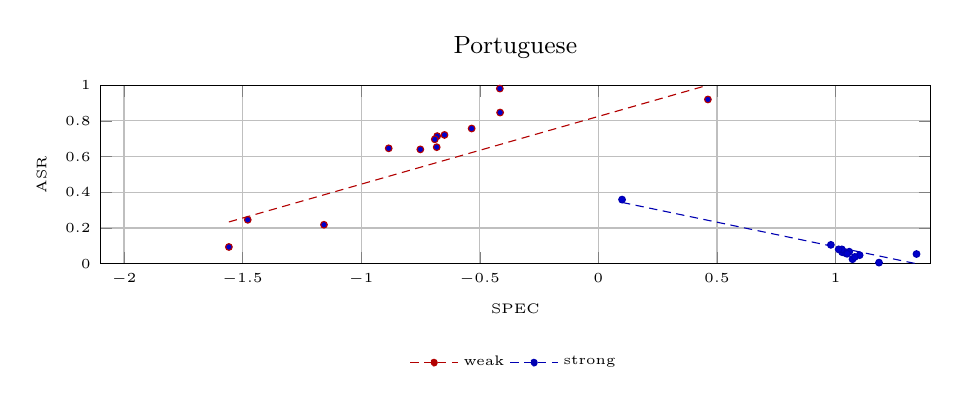
\begin{tikzpicture}
\begin{axis}[width=\linewidth,height=3.85cm,grid=both,
title={Portuguese},xlabel={SPEC},ylabel={ASR},
xmin=-2.1,xmax=1.4,ymin=0,ymax=1,
tick label style={font=\tiny},label style={font=\tiny},title style={font=\small},
legend style={font=\tiny,at={(0.5,-0.45)},anchor=north,draw=none,fill=none,legend columns=2}]
\addplot+[forget plot,only marks,mark=*,mark size=1.2pt,red!70!black] coordinates {(-1.4783,0.2460) (-0.6816,0.6527) (-0.6796,0.7147) (-0.4154,0.9808) (-1.1569,0.2184) (-0.5343,0.7572) (-0.8840,0.6463) (0.4617,0.9199) (-0.6488,0.7212) (-0.4143,0.8466) (-1.5577,0.0939) (-0.6897,0.6968) (-0.7506,0.6403)};
\addplot+[forget plot,no markers,densely dashed,red!70!black] coordinates {(-1.5577,0.2340) (0.4617,1.0000)};
\addplot+[forget plot,only marks,mark=*,mark size=1.2pt,blue!70!black] coordinates {(1.0279,0.0647) (1.0576,0.0675) (1.0442,0.0581) (1.1830,0.0064) (0.9800,0.1058) (1.0714,0.0256) (1.0266,0.0804) (1.3412,0.0545) (1.1013,0.0481) (1.0810,0.0383) (0.0998,0.3592) (1.0129,0.0806) (1.0490,0.0561)};
\addplot+[forget plot,no markers,densely dashed,blue!70!black] coordinates {(0.0998,0.3434) (1.3412,0.0000)};
\addlegendimage{densely dashed,mark=*,mark size=1.2pt,red!70!black}
\addlegendentry{weak}
\addlegendimage{densely dashed,mark=*,mark size=1.2pt,blue!70!black}
\addlegendentry{strong}
\end{axis}
\end{tikzpicture}
\end{minipage}
\hfill\begin{minipage}{0.48\linewidth}\centering
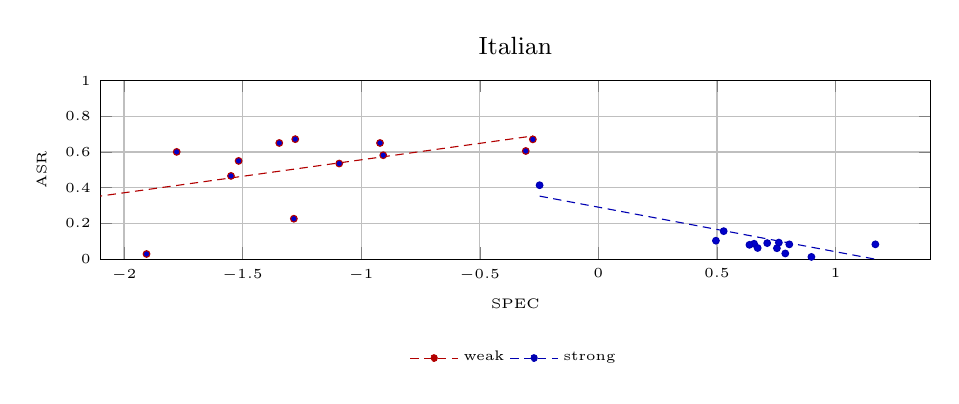
\begin{tikzpicture}
\begin{axis}[width=\linewidth,height=3.85cm,grid=both,
title={Italian},xlabel={SPEC},ylabel={ASR},
xmin=-2.1,xmax=1.4,ymin=0,ymax=1,
tick label style={font=\tiny},label style={font=\tiny},title style={font=\small},
legend style={font=\tiny,at={(0.5,-0.45)},anchor=north,draw=none,fill=none,legend columns=2}]
\addplot+[forget plot,only marks,mark=*,mark size=1.2pt,red!70!black] coordinates {(-1.2838,0.2265) (-1.5489,0.4662) (-0.9070,0.5820) (-0.9206,0.6506) (-2.1846,0.3754) (-0.2762,0.6709) (-1.0926,0.5355) (-1.2779,0.6720) (-0.3061,0.6058) (-1.3453,0.6506) (-1.9049,0.0291) (-1.5167,0.5502) (-1.7777,0.6007)};
\addplot+[forget plot,no markers,densely dashed,red!70!black] coordinates {(-2.1846,0.3377) (-0.2762,0.6899)};
\addplot+[forget plot,only marks,mark=*,mark size=1.2pt,blue!70!black] coordinates {(0.4955,0.1036) (0.7117,0.0900) (0.6564,0.0865) (0.8980,0.0128) (0.5282,0.1570) (1.1677,0.0831) (0.6368,0.0804) (0.7608,0.0929) (0.7879,0.0321) (0.8049,0.0831) (-0.2478,0.4142) (0.7526,0.0613) (0.6714,0.0627)};
\addplot+[forget plot,no markers,densely dashed,blue!70!black] coordinates {(-0.2478,0.3531) (1.1677,0.0000)};
\addlegendimage{densely dashed,mark=*,mark size=1.2pt,red!70!black}
\addlegendentry{weak}
\addlegendimage{densely dashed,mark=*,mark size=1.2pt,blue!70!black}
\addlegendentry{strong}
\end{axis}
\end{tikzpicture}
\end{minipage}
\vspace{0.7cm}
\begin{minipage}{0.48\linewidth}\centering
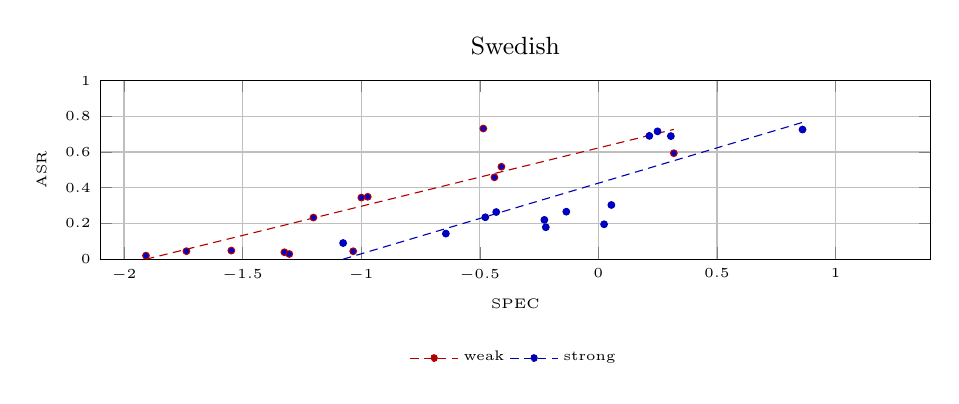
\begin{tikzpicture}
\begin{axis}[width=\linewidth,height=3.85cm,grid=both,
title={Swedish},xlabel={SPEC},ylabel={ASR},
xmin=-2.1,xmax=1.4,ymin=0,ymax=1,
tick label style={font=\tiny},label style={font=\tiny},title style={font=\small},
legend style={font=\tiny,at={(0.5,-0.45)},anchor=north,draw=none,fill=none,legend columns=2}]
\addplot+[forget plot,only marks,mark=*,mark size=1.2pt,red!70!black] coordinates {(-1.3237,0.0388) (-1.5474,0.0482) (-0.4383,0.4583) (-0.4850,0.7316) (-1.0337,0.0444) (-1.2013,0.2332) (-0.4087,0.5177) (-0.9724,0.3494) (-1.7367,0.0449) (-0.9992,0.3450) (-1.3031,0.0291) (0.3181,0.5935) (-1.9072,0.0198)};
\addplot+[forget plot,no markers,densely dashed,red!70!black] coordinates {(-1.9072,0.0000) (0.3181,0.7267)};
\addplot+[forget plot,only marks,mark=*,mark size=1.2pt,blue!70!black] coordinates {(-0.2277,0.2201) (-0.4768,0.2347) (0.3055,0.6891) (0.2493,0.7157) (-0.6430,0.1433) (-0.2216,0.1789) (0.2148,0.6903) (0.0240,0.1955) (-0.1352,0.2660) (0.0547,0.3035) (-1.0761,0.0906) (0.8606,0.7258) (-0.4307,0.2640)};
\addplot+[forget plot,no markers,densely dashed,blue!70!black] coordinates {(-1.0761,0.0000) (0.8606,0.7659)};
\addlegendimage{densely dashed,mark=*,mark size=1.2pt,red!70!black}
\addlegendentry{weak}
\addlegendimage{densely dashed,mark=*,mark size=1.2pt,blue!70!black}
\addlegendentry{strong}
\end{axis}
\end{tikzpicture}
\end{minipage}
\hfill\begin{minipage}{0.48\linewidth}\centering
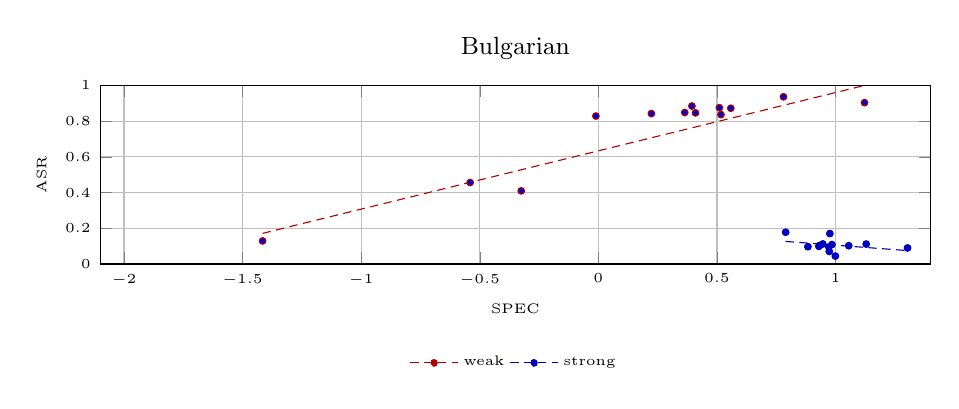
\begin{tikzpicture}
\begin{axis}[width=\linewidth,height=3.85cm,grid=both,
title={Bulgarian},xlabel={SPEC},ylabel={ASR},
xmin=-2.1,xmax=1.4,ymin=0,ymax=1,
tick label style={font=\tiny},label style={font=\tiny},title style={font=\small},
legend style={font=\tiny,at={(0.5,-0.45)},anchor=north,draw=none,fill=none,legend columns=2}]
\addplot+[forget plot,only marks,mark=*,mark size=1.2pt,red!70!black] coordinates {(-0.5405,0.4563) (1.1219,0.9035) (0.4094,0.8462) (0.7803,0.9361) (-0.3252,0.4096) (0.5102,0.8754) (0.2235,0.8424) (0.5168,0.8365) (0.3943,0.8846) (0.5583,0.8722) (-1.4156,0.1294) (0.3641,0.8484) (-0.0105,0.8284)};
\addplot+[forget plot,no markers,densely dashed,red!70!black] coordinates {(-1.4156,0.1718) (1.1219,1.0000)};
\addplot+[forget plot,only marks,mark=*,mark size=1.2pt,blue!70!black] coordinates {(0.8833,0.0971) (1.3034,0.0900) (1.0554,0.1026) (1.1290,0.1118) (0.9758,0.1706) (0.9990,0.0447) (0.9461,0.1125) (0.9845,0.1090) (0.9732,0.0705) (0.9711,0.0958) (0.7893,0.1780) (0.9323,0.1037) (0.9296,0.0990)};
\addplot+[forget plot,no markers,densely dashed,blue!70!black] coordinates {(0.7893,0.1267) (1.3034,0.0752)};
\addlegendimage{densely dashed,mark=*,mark size=1.2pt,red!70!black}
\addlegendentry{weak}
\addlegendimage{densely dashed,mark=*,mark size=1.2pt,blue!70!black}
\addlegendentry{strong}
\end{axis}
\end{tikzpicture}
\end{minipage}
\vspace{0.7cm}

\label{fig:spec-vs-asr}
\fonte{Prepared by the author (2026).}
\end{figure}
}

\newcommand{\TokenizerDiagnosticsFigure}{%
\begin{landscape}
\begin{figure}[p]
\centering
\caption[Mean token inflation by model and attack language]{Mean token inflation by model and attack language: the attack-language prompt's token count relative to the same prompt in the model's aligned language, after applying its chat template. Shading uses one log scale for all models. Bold values mark each model's aligned language. Dashes indicate unavailable measurements. The English reference is descriptive.}
\begingroup
\definecolor{UrielClose}{HTML}{355C7D}
\definecolor{UrielMiddle}{HTML}{4ECDC4}
\definecolor{UrielFar}{HTML}{F0932B}
\scriptsize
\setlength{\tabcolsep}{3.2pt}
\renewcommand{\arraystretch}{1.18}
\begin{adjustbox}{width=0.9\linewidth,center}
\begin{tabular}{>{\raggedright\arraybackslash}p{3.75cm}|*{13}{>{\centering\arraybackslash}p{0.88cm}}}
\hline
\textbf{Model} & \cellcolor[HTML]{F7D7CF}\textbf{\texttt{ita}} & \cellcolor[HTML]{F7D7CF}\textbf{\texttt{por}} & \cellcolor[HTML]{F7D7CF}\textbf{\texttt{spa}} & \cellcolor[HTML]{D6E6F6}\textbf{\texttt{eng}} & \cellcolor[HTML]{D6E6F6}\textbf{\texttt{dan}} & \cellcolor[HTML]{D6E6F6}\textbf{\texttt{nor}} & \cellcolor[HTML]{D6E6F6}\textbf{\texttt{swe}} & \cellcolor[HTML]{D8F0E1}\textbf{\texttt{fin}} & \cellcolor[HTML]{E8DDF5}\textbf{\texttt{bul}} & \cellcolor[HTML]{E8DDF5}\textbf{\texttt{rus}} & \cellcolor[HTML]{E8DDF5}\textbf{\texttt{ukr}} & \cellcolor[HTML]{F8E2C2}\textbf{\texttt{ara}} & \cellcolor[HTML]{DCEBC8}\textbf{\texttt{swa}} \\
\hline
\cellcolor[HTML]{F7D7CF}\textbf{\mbox{Sagui-7B (\texttt{por})}} & \cellcolor[HTML]{4295A1}\textcolor{black}{1.00} & \cellcolor[HTML]{4295A1}\textcolor{black}{\textbf{1.00}} & \cellcolor[HTML]{4296A2}\textcolor{black}{1.01} & \cellcolor[HTML]{3A728B}\textcolor{white}{0.79} & \cellcolor[HTML]{44A1A9}\textcolor{black}{1.08} & \cellcolor[HTML]{44A0A8}\textcolor{black}{1.07} & \cellcolor[HTML]{439AA4}\textcolor{black}{1.03} & \cellcolor[HTML]{48B0B2}\textcolor{black}{1.19} & \cellcolor[HTML]{47AFB1}\textcolor{black}{1.18} & \cellcolor[HTML]{45A4AA}\textcolor{black}{1.10} & \cellcolor[HTML]{47ACAF}\textcolor{black}{1.16} & \cellcolor[HTML]{BBDDA0}\textcolor{black}{1.92} & \cellcolor[HTML]{49B7B6}\textcolor{black}{1.24} \\
\cellcolor[HTML]{F7D7CF}\textbf{\mbox{Sabi\'a-3 (\texttt{por})}} & \cellcolor[HTML]{E6E6E6}\textemdash & \cellcolor[HTML]{E6E6E6}\textemdash & \cellcolor[HTML]{E6E6E6}\textemdash & \cellcolor[HTML]{E6E6E6}\textemdash & \cellcolor[HTML]{E6E6E6}\textemdash & \cellcolor[HTML]{E6E6E6}\textemdash & \cellcolor[HTML]{E6E6E6}\textemdash & \cellcolor[HTML]{E6E6E6}\textemdash & \cellcolor[HTML]{E6E6E6}\textemdash & \cellcolor[HTML]{E6E6E6}\textemdash & \cellcolor[HTML]{E6E6E6}\textemdash & \cellcolor[HTML]{E6E6E6}\textemdash & \cellcolor[HTML]{E6E6E6}\textemdash \\
\hline
\cellcolor[HTML]{F7D7CF}\textbf{\mbox{LLaMAntino-2 (\texttt{ita})}} & \cellcolor[HTML]{4295A1}\textcolor{black}{\textbf{1.00}} & \cellcolor[HTML]{4295A1}\textcolor{black}{1.00} & \cellcolor[HTML]{4296A1}\textcolor{black}{1.00} & \cellcolor[HTML]{3F8B9B}\textcolor{black}{0.94} & \cellcolor[HTML]{4399A3}\textcolor{black}{1.03} & \cellcolor[HTML]{4299A3}\textcolor{black}{1.02} & \cellcolor[HTML]{4297A2}\textcolor{black}{1.01} & \cellcolor[HTML]{449EA7}\textcolor{black}{1.06} & \cellcolor[HTML]{449EA6}\textcolor{black}{1.06} & \cellcolor[HTML]{439AA4}\textcolor{black}{1.03} & \cellcolor[HTML]{439DA6}\textcolor{black}{1.05} & \cellcolor[HTML]{4ABCB9}\textcolor{black}{1.29} & \cellcolor[HTML]{44A1A8}\textcolor{black}{1.08} \\
\cellcolor[HTML]{F7D7CF}\textbf{\mbox{ANITA (\texttt{ita})}} & \cellcolor[HTML]{4295A1}\textcolor{black}{\textbf{1.00}} & \cellcolor[HTML]{408D9C}\textcolor{black}{0.95} & \cellcolor[HTML]{408C9B}\textcolor{black}{0.94} & \cellcolor[HTML]{366281}\textcolor{white}{0.72} & \cellcolor[HTML]{449EA6}\textcolor{black}{1.06} & \cellcolor[HTML]{439AA4}\textcolor{black}{1.03} & \cellcolor[HTML]{4298A3}\textcolor{black}{1.02} & \cellcolor[HTML]{48B1B2}\textcolor{black}{1.20} & \cellcolor[HTML]{49B8B7}\textcolor{black}{1.26} & \cellcolor[HTML]{4298A2}\textcolor{black}{1.02} & \cellcolor[HTML]{449FA7}\textcolor{black}{1.07} & \cellcolor[HTML]{4399A3}\textcolor{black}{1.03} & \cellcolor[HTML]{49B7B6}\textcolor{black}{1.24} \\
\hline
\cellcolor[HTML]{D6E6F6}\textbf{\mbox{GPT-SW3 (\texttt{swe})}} & \cellcolor[HTML]{6BD1BB}\textcolor{black}{1.55} & \cellcolor[HTML]{7AD3B6}\textcolor{black}{1.61} & \cellcolor[HTML]{84D5B2}\textcolor{black}{1.66} & \cellcolor[HTML]{4295A1}\textcolor{black}{1.00} & \cellcolor[HTML]{449FA7}\textcolor{black}{1.07} & \cellcolor[HTML]{439CA5}\textcolor{black}{1.05} & \cellcolor[HTML]{4295A1}\textcolor{black}{\textbf{1.00}} & \cellcolor[HTML]{86D5B2}\textcolor{black}{1.67} & \cellcolor[HTML]{F19B34}\textcolor{black}{3.38} & \cellcolor[HTML]{F09831}\textcolor{black}{3.44} & \cellcolor[HTML]{F0932B}\textcolor{black}{3.54} & \cellcolor[HTML]{F19F3A}\textcolor{black}{3.31} & \cellcolor[HTML]{A8DAA7}\textcolor{black}{1.82} \\
\cellcolor[HTML]{D6E6F6}\textbf{\mbox{AI Sweden (\texttt{swe})}} & \cellcolor[HTML]{4194A0}\textcolor{black}{0.99} & \cellcolor[HTML]{408C9B}\textcolor{black}{0.94} & \cellcolor[HTML]{3F8B9B}\textcolor{black}{0.94} & \cellcolor[HTML]{366080}\textcolor{white}{0.71} & \cellcolor[HTML]{439CA5}\textcolor{black}{1.04} & \cellcolor[HTML]{4298A3}\textcolor{black}{1.02} & \cellcolor[HTML]{4295A1}\textcolor{black}{\textbf{1.00}} & \cellcolor[HTML]{47AEB1}\textcolor{black}{1.18} & \cellcolor[HTML]{49B6B5}\textcolor{black}{1.24} & \cellcolor[HTML]{4296A1}\textcolor{black}{1.00} & \cellcolor[HTML]{439DA6}\textcolor{black}{1.05} & \cellcolor[HTML]{4297A2}\textcolor{black}{1.01} & \cellcolor[HTML]{49B5B5}\textcolor{black}{1.23} \\
\hline
\cellcolor[HTML]{E8DDF5}\textbf{\mbox{BgGPT-7B (\texttt{bul})}} & \cellcolor[HTML]{48B0B2}\textcolor{black}{1.19} & \cellcolor[HTML]{48B0B2}\textcolor{black}{1.19} & \cellcolor[HTML]{48B2B3}\textcolor{black}{1.21} & \cellcolor[HTML]{3B778E}\textcolor{white}{0.82} & \cellcolor[HTML]{4ABCBA}\textcolor{black}{1.29} & \cellcolor[HTML]{4ABBB9}\textcolor{black}{1.28} & \cellcolor[HTML]{48B0B2}\textcolor{black}{1.19} & \cellcolor[HTML]{4FCDC4}\textcolor{black}{1.44} & \cellcolor[HTML]{4295A1}\textcolor{black}{\textbf{1.00}} & \cellcolor[HTML]{4ABCB9}\textcolor{black}{1.28} & \cellcolor[HTML]{4DC7C0}\textcolor{black}{1.38} & \cellcolor[HTML]{F5D67B}\textcolor{black}{2.43} & \cellcolor[HTML]{5ACFC0}\textcolor{black}{1.49} \\
\cellcolor[HTML]{E8DDF5}\textbf{\mbox{BgGPT-Gemma (\texttt{bul})}} & \cellcolor[HTML]{3B758D}\textcolor{white}{0.81} & \cellcolor[HTML]{396F89}\textcolor{white}{0.78} & \cellcolor[HTML]{386B87}\textcolor{white}{0.76} & \cellcolor[HTML]{355C7D}\textcolor{white}{0.69} & \cellcolor[HTML]{3D8194}\textcolor{white}{0.88} & \cellcolor[HTML]{3D7E92}\textcolor{white}{0.86} & \cellcolor[HTML]{3C7C91}\textcolor{white}{0.85} & \cellcolor[HTML]{41909E}\textcolor{black}{0.97} & \cellcolor[HTML]{4295A1}\textcolor{black}{\textbf{1.00}} & \cellcolor[HTML]{3C7C91}\textcolor{white}{0.85} & \cellcolor[HTML]{4296A1}\textcolor{black}{1.00} & \cellcolor[HTML]{3E8496}\textcolor{white}{0.89} & \cellcolor[HTML]{4297A2}\textcolor{black}{1.01} \\
\hline
\cellcolor[HTML]{D6E6F6}\textbf{\mbox{English reference (\texttt{eng})}} & \cellcolor[HTML]{49B7B6}\textcolor{black}{1.24} & \cellcolor[HTML]{48B1B2}\textcolor{black}{1.20} & \cellcolor[HTML]{48B0B2}\textcolor{black}{1.19} & \cellcolor[HTML]{4295A1}\textcolor{black}{\textbf{1.00}} & \cellcolor[HTML]{4ABCB9}\textcolor{black}{1.29} & \cellcolor[HTML]{4AB9B8}\textcolor{black}{1.27} & \cellcolor[HTML]{49B8B7}\textcolor{black}{1.26} & \cellcolor[HTML]{4DCAC2}\textcolor{black}{1.41} & \cellcolor[HTML]{53CEC2}\textcolor{black}{1.46} & \cellcolor[HTML]{49B8B7}\textcolor{black}{1.25} & \cellcolor[HTML]{4ABDBA}\textcolor{black}{1.30} & \cellcolor[HTML]{49B9B7}\textcolor{black}{1.26} & \cellcolor[HTML]{50CDC3}\textcolor{black}{1.45} \\
\hline
\end{tabular}
\end{adjustbox}
\vspace{0.55em}
\begin{tikzpicture}[x=1cm,y=0.28cm]
\fill[UrielClose] (0,0) rectangle (0.55,1);\node[anchor=west,font=\scriptsize] at (0.65,0.5) {lower};
\fill[UrielMiddle] (2.1,0) rectangle (2.65,1);\node[anchor=west,font=\scriptsize] at (2.75,0.5) {intermediate};
\fill[UrielFar] (5.0,0) rectangle (5.55,1);\node[anchor=west,font=\scriptsize] at (5.65,0.5) {higher};
\node[anchor=west,font=\scriptsize] at (8.25,0.5) {Rows show each model with its aligned language; columns are grouped by broad family as in Table~\ref{tab:urielplus-distances}.};
\end{tikzpicture}
\label{fig:tokenizer-diagnostics}
\par\fonte{Prepared by the author (2026).}
\endgroup
\end{figure}
\end{landscape}
}

\newcommand{\TokensPerCharacterFigure}{%
\begin{landscape}
\begin{figure}[p]
\centering
\caption[Mean tokens per character by model and attack language]{Mean tokens per character by model and attack language. Each value averages prompt-level chat-template token counts divided by the number of characters in the attack-language prompt before chat-template rendering. Characters are Unicode code points, not UTF-8 bytes. Shading is normalized separately within each model's row. Bold values mark each model's aligned language. Dashes indicate unavailable measurements. The English reference is descriptive. These values reflect tokenizer segmentation and template overhead, not comprehension or safety.}
\begingroup
\definecolor{UrielClose}{HTML}{355C7D}
\definecolor{UrielMiddle}{HTML}{4ECDC4}
\definecolor{UrielFar}{HTML}{F0932B}
\scriptsize
\setlength{\tabcolsep}{3.2pt}
\renewcommand{\arraystretch}{1.18}
\begin{adjustbox}{width=0.9\linewidth,center}
\begin{tabular}{>{\raggedright\arraybackslash}p{3.75cm}|*{13}{>{\centering\arraybackslash}p{0.88cm}}}
\hline
\textbf{Model} & \cellcolor[HTML]{F7D7CF}\textbf{\texttt{ita}} & \cellcolor[HTML]{F7D7CF}\textbf{\texttt{por}} & \cellcolor[HTML]{F7D7CF}\textbf{\texttt{spa}} & \cellcolor[HTML]{D6E6F6}\textbf{\texttt{eng}} & \cellcolor[HTML]{D6E6F6}\textbf{\texttt{dan}} & \cellcolor[HTML]{D6E6F6}\textbf{\texttt{nor}} & \cellcolor[HTML]{D6E6F6}\textbf{\texttt{swe}} & \cellcolor[HTML]{D8F0E1}\textbf{\texttt{fin}} & \cellcolor[HTML]{E8DDF5}\textbf{\texttt{bul}} & \cellcolor[HTML]{E8DDF5}\textbf{\texttt{rus}} & \cellcolor[HTML]{E8DDF5}\textbf{\texttt{ukr}} & \cellcolor[HTML]{F8E2C2}\textbf{\texttt{ara}} & \cellcolor[HTML]{DCEBC8}\textbf{\texttt{swa}} \\
\hline
\cellcolor[HTML]{F7D7CF}\textbf{\mbox{Sagui-7B (\texttt{por})}} & \cellcolor[HTML]{386C87}\textcolor{white}{0.457} & \cellcolor[HTML]{3A718A}\textcolor{white}{\textbf{0.473}} & \cellcolor[HTML]{396C87}\textcolor{white}{0.459} & \cellcolor[HTML]{355C7D}\textcolor{white}{0.412} & \cellcolor[HTML]{3D8295}\textcolor{white}{0.523} & \cellcolor[HTML]{3E8396}\textcolor{white}{0.526} & \cellcolor[HTML]{3D8094}\textcolor{white}{0.518} & \cellcolor[HTML]{439BA5}\textcolor{black}{0.597} & \cellcolor[HTML]{4194A0}\textcolor{black}{0.576} & \cellcolor[HTML]{3D8194}\textcolor{white}{0.521} & \cellcolor[HTML]{40909D}\textcolor{black}{0.563} & \cellcolor[HTML]{F0932B}\textcolor{black}{1.145} & \cellcolor[HTML]{4297A2}\textcolor{black}{0.583} \\
\cellcolor[HTML]{F7D7CF}\textbf{\mbox{Sabi\'a-3 (\texttt{por})}} & \cellcolor[HTML]{E6E6E6}\textemdash & \cellcolor[HTML]{E6E6E6}\textemdash & \cellcolor[HTML]{E6E6E6}\textemdash & \cellcolor[HTML]{E6E6E6}\textemdash & \cellcolor[HTML]{E6E6E6}\textemdash & \cellcolor[HTML]{E6E6E6}\textemdash & \cellcolor[HTML]{E6E6E6}\textemdash & \cellcolor[HTML]{E6E6E6}\textemdash & \cellcolor[HTML]{E6E6E6}\textemdash & \cellcolor[HTML]{E6E6E6}\textemdash & \cellcolor[HTML]{E6E6E6}\textemdash & \cellcolor[HTML]{E6E6E6}\textemdash & \cellcolor[HTML]{E6E6E6}\textemdash \\
\hline
\cellcolor[HTML]{F7D7CF}\textbf{\mbox{LLaMAntino-2 (\texttt{ita})}} & \cellcolor[HTML]{355E7E}\textcolor{white}{\textbf{1.657}} & \cellcolor[HTML]{386A86}\textcolor{white}{1.710} & \cellcolor[HTML]{355C7D}\textcolor{white}{1.649} & \cellcolor[HTML]{3B768D}\textcolor{white}{1.761} & \cellcolor[HTML]{3C7C91}\textcolor{white}{1.788} & \cellcolor[HTML]{3D8295}\textcolor{white}{1.811} & \cellcolor[HTML]{3F8999}\textcolor{black}{1.843} & \cellcolor[HTML]{439CA5}\textcolor{black}{1.926} & \cellcolor[HTML]{408C9B}\textcolor{black}{1.857} & \cellcolor[HTML]{3B768D}\textcolor{white}{1.761} & \cellcolor[HTML]{3F8999}\textcolor{black}{1.843} & \cellcolor[HTML]{F0932B}\textcolor{black}{2.729} & \cellcolor[HTML]{3E8496}\textcolor{white}{1.820} \\
\cellcolor[HTML]{F7D7CF}\textbf{\mbox{ANITA (\texttt{ita})}} & \cellcolor[HTML]{49B6B5}\textcolor{black}{\textbf{0.360}} & \cellcolor[HTML]{46AAAE}\textcolor{black}{0.351} & \cellcolor[HTML]{4297A2}\textcolor{black}{0.336} & \cellcolor[HTML]{355C7D}\textcolor{white}{0.290} & \cellcolor[HTML]{91D7AE}\textcolor{black}{0.400} & \cellcolor[HTML]{87D5B1}\textcolor{black}{0.396} & \cellcolor[HTML]{92D7AE}\textcolor{black}{0.400} & \cellcolor[HTML]{F2AD4A}\textcolor{black}{0.469} & \cellcolor[HTML]{F1A03B}\textcolor{black}{0.478} & \cellcolor[HTML]{4DCBC3}\textcolor{black}{0.376} & \cellcolor[HTML]{AADAA6}\textcolor{black}{0.407} & \cellcolor[HTML]{F0932B}\textcolor{black}{0.487} & \cellcolor[HTML]{F3BE5E}\textcolor{black}{0.458} \\
\hline
\cellcolor[HTML]{D6E6F6}\textbf{\mbox{GPT-SW3 (\texttt{swe})}} & \cellcolor[HTML]{3C7E92}\textcolor{white}{0.381} & \cellcolor[HTML]{3E8698}\textcolor{white}{0.408} & \cellcolor[HTML]{3E8597}\textcolor{white}{0.405} & \cellcolor[HTML]{355D7E}\textcolor{white}{0.278} & \cellcolor[HTML]{355E7E}\textcolor{white}{0.279} & \cellcolor[HTML]{355D7E}\textcolor{white}{0.278} & \cellcolor[HTML]{355C7D}\textcolor{white}{\textbf{0.274}} & \cellcolor[HTML]{4193A0}\textcolor{black}{0.450} & \cellcolor[HTML]{F5D87D}\textcolor{black}{0.884} & \cellcolor[HTML]{F5DD83}\textcolor{black}{0.871} & \cellcolor[HTML]{F4CA6D}\textcolor{black}{0.922} & \cellcolor[HTML]{F0932B}\textcolor{black}{1.072} & \cellcolor[HTML]{4297A2}\textcolor{black}{0.460} \\
\cellcolor[HTML]{D6E6F6}\textbf{\mbox{AI Sweden (\texttt{swe})}} & \cellcolor[HTML]{49B6B5}\textcolor{black}{0.360} & \cellcolor[HTML]{46AAAE}\textcolor{black}{0.351} & \cellcolor[HTML]{4297A2}\textcolor{black}{0.336} & \cellcolor[HTML]{355C7D}\textcolor{white}{0.290} & \cellcolor[HTML]{91D7AE}\textcolor{black}{0.400} & \cellcolor[HTML]{88D5B1}\textcolor{black}{0.397} & \cellcolor[HTML]{92D7AE}\textcolor{black}{\textbf{0.400}} & \cellcolor[HTML]{F2AD4A}\textcolor{black}{0.469} & \cellcolor[HTML]{F1A03B}\textcolor{black}{0.478} & \cellcolor[HTML]{4DCBC3}\textcolor{black}{0.376} & \cellcolor[HTML]{AADAA6}\textcolor{black}{0.407} & \cellcolor[HTML]{F0932B}\textcolor{black}{0.487} & \cellcolor[HTML]{F3BE5E}\textcolor{black}{0.458} \\
\hline
\cellcolor[HTML]{E8DDF5}\textbf{\mbox{BgGPT-7B (\texttt{bul})}} & \cellcolor[HTML]{3B798F}\textcolor{white}{0.374} & \cellcolor[HTML]{3C7D92}\textcolor{white}{0.385} & \cellcolor[HTML]{3C7A90}\textcolor{white}{0.376} & \cellcolor[HTML]{355C7D}\textcolor{white}{0.291} & \cellcolor[HTML]{408C9B}\textcolor{black}{0.428} & \cellcolor[HTML]{408D9C}\textcolor{black}{0.430} & \cellcolor[HTML]{3E8697}\textcolor{white}{0.409} & \cellcolor[HTML]{45A4AA}\textcolor{black}{0.496} & \cellcolor[HTML]{396D88}\textcolor{white}{\textbf{0.340}} & \cellcolor[HTML]{3F8899}\textcolor{black}{0.417} & \cellcolor[HTML]{4298A3}\textcolor{black}{0.462} & \cellcolor[HTML]{F0932B}\textcolor{black}{1.002} & \cellcolor[HTML]{449EA7}\textcolor{black}{0.479} \\
\cellcolor[HTML]{E8DDF5}\textbf{\mbox{BgGPT-Gemma (\texttt{bul})}} & \cellcolor[HTML]{3C7C91}\textcolor{white}{0.297} & \cellcolor[HTML]{3B778E}\textcolor{white}{0.293} & \cellcolor[HTML]{355C7D}\textcolor{white}{0.277} & \cellcolor[HTML]{376683}\textcolor{white}{0.283} & \cellcolor[HTML]{4BC0BC}\textcolor{black}{0.339} & \cellcolor[HTML]{4ABDBA}\textcolor{black}{0.337} & \cellcolor[HTML]{4ECBC3}\textcolor{black}{0.346} & \cellcolor[HTML]{F6E289}\textcolor{black}{0.390} & \cellcolor[HTML]{F5DD84}\textcolor{black}{\textbf{0.393}} & \cellcolor[HTML]{45A3AA}\textcolor{black}{0.321} & \cellcolor[HTML]{F6DE85}\textcolor{black}{0.392} & \cellcolor[HTML]{F0932B}\textcolor{black}{0.432} & \cellcolor[HTML]{D6E097}\textcolor{black}{0.381} \\
\hline
\cellcolor[HTML]{D6E6F6}\textbf{\mbox{English reference (\texttt{eng})}} & \cellcolor[HTML]{408D9C}\textcolor{black}{0.558} & \cellcolor[HTML]{3F8A9A}\textcolor{black}{0.556} & \cellcolor[HTML]{3A728B}\textcolor{white}{0.533} & \cellcolor[HTML]{355C7D}\textcolor{white}{\textbf{0.513}} & \cellcolor[HTML]{4CC2BD}\textcolor{black}{0.609} & \cellcolor[HTML]{4CC2BD}\textcolor{black}{0.609} & \cellcolor[HTML]{4ECDC4}\textcolor{black}{0.619} & \cellcolor[HTML]{F5DD83}\textcolor{black}{0.690} & \cellcolor[HTML]{F5DC83}\textcolor{black}{0.690} & \cellcolor[HTML]{45A5AB}\textcolor{black}{0.582} & \cellcolor[HTML]{4FCDC4}\textcolor{black}{0.619} & \cellcolor[HTML]{F0932B}\textcolor{black}{0.749} & \cellcolor[HTML]{C1DD9E}\textcolor{black}{0.663} \\
\hline
\end{tabular}
\end{adjustbox}
\vspace{0.55em}
\begin{tikzpicture}[x=1cm,y=0.28cm]
\fill[UrielClose] (0,0) rectangle (0.55,1);\node[anchor=west,font=\scriptsize] at (0.65,0.5) {lower};
\fill[UrielMiddle] (2.1,0) rectangle (2.65,1);\node[anchor=west,font=\scriptsize] at (2.75,0.5) {intermediate};
\fill[UrielFar] (5.0,0) rectangle (5.55,1);\node[anchor=west,font=\scriptsize] at (5.65,0.5) {higher};
\node[anchor=west,font=\scriptsize] at (8.25,0.5) {Shading compares languages within a model, not across models.};
\end{tikzpicture}
\label{fig:tokens-per-character}
\par\fonte{Prepared by the author (2026).}
\endgroup
\end{figure}
\end{landscape}
}
